\documentclass[../main.tex]{subfiles}
\usepackage{slashed}
\usepackage[table]{xcolor}
\usepackage{hhline}
\usepackage{lipsum}

\let\Bbbk\relax
\usepackage{amsmath}
\usepackage{amsfonts}

\begin{document}
\setchapterimage[6.5cm]{images/feynman-1.jpg}
\setchapterpreamble[u]{\margintoc}
\chapter[Il concetto di Divergenza in QFT]{Il concetto di Divergenza in QFT}
%\labch{divergence}
\label{ch:divergence}

\fboxsep =1pt % separazione per i box

\section{Introduzione}
Lo scopo di questa parte è quello di imparare a trattare gli \textit{infiniti} che affliggono i calcoli delle osservabili in teoria dei campi.\\
Quando si prova a calcolare un particolare elemento di matrice, infatti, è possibile espandere il calcolo in serie rispetto alla costante di struttura fine $\alpha$, i cui termini sono di fatto rappresentabili con dei diagrammi di Feynman.\\
In maniera ingenua, avvalendosi del fatto che $\alpha$ ha valore molto piccolo, ci si può accontentare del prim'ordine (o \textbf{Tree-Level}); tuttavia, se si procede con il calcolo degli ordini successivi (\textbf{Loops}), ci si accorge che i loro contributi presentano un fattore moltiplicativo che tende ad infinito, e questo è un bel problema.\\



\section{Grado di Divergenza}
Partiamo innanzitutto con alcune utili nomenclature riguardo i diagrammi di Feynman (composti da linee esterne, vertici e propagatori):
\marginnote{\underline{\textbf{Nota:}} Un diagramma di questo tipo \textbf{NON} è 1PI, infatti separandolo tagliando il propagatore al centro si ottengono due diagrammi distinti. 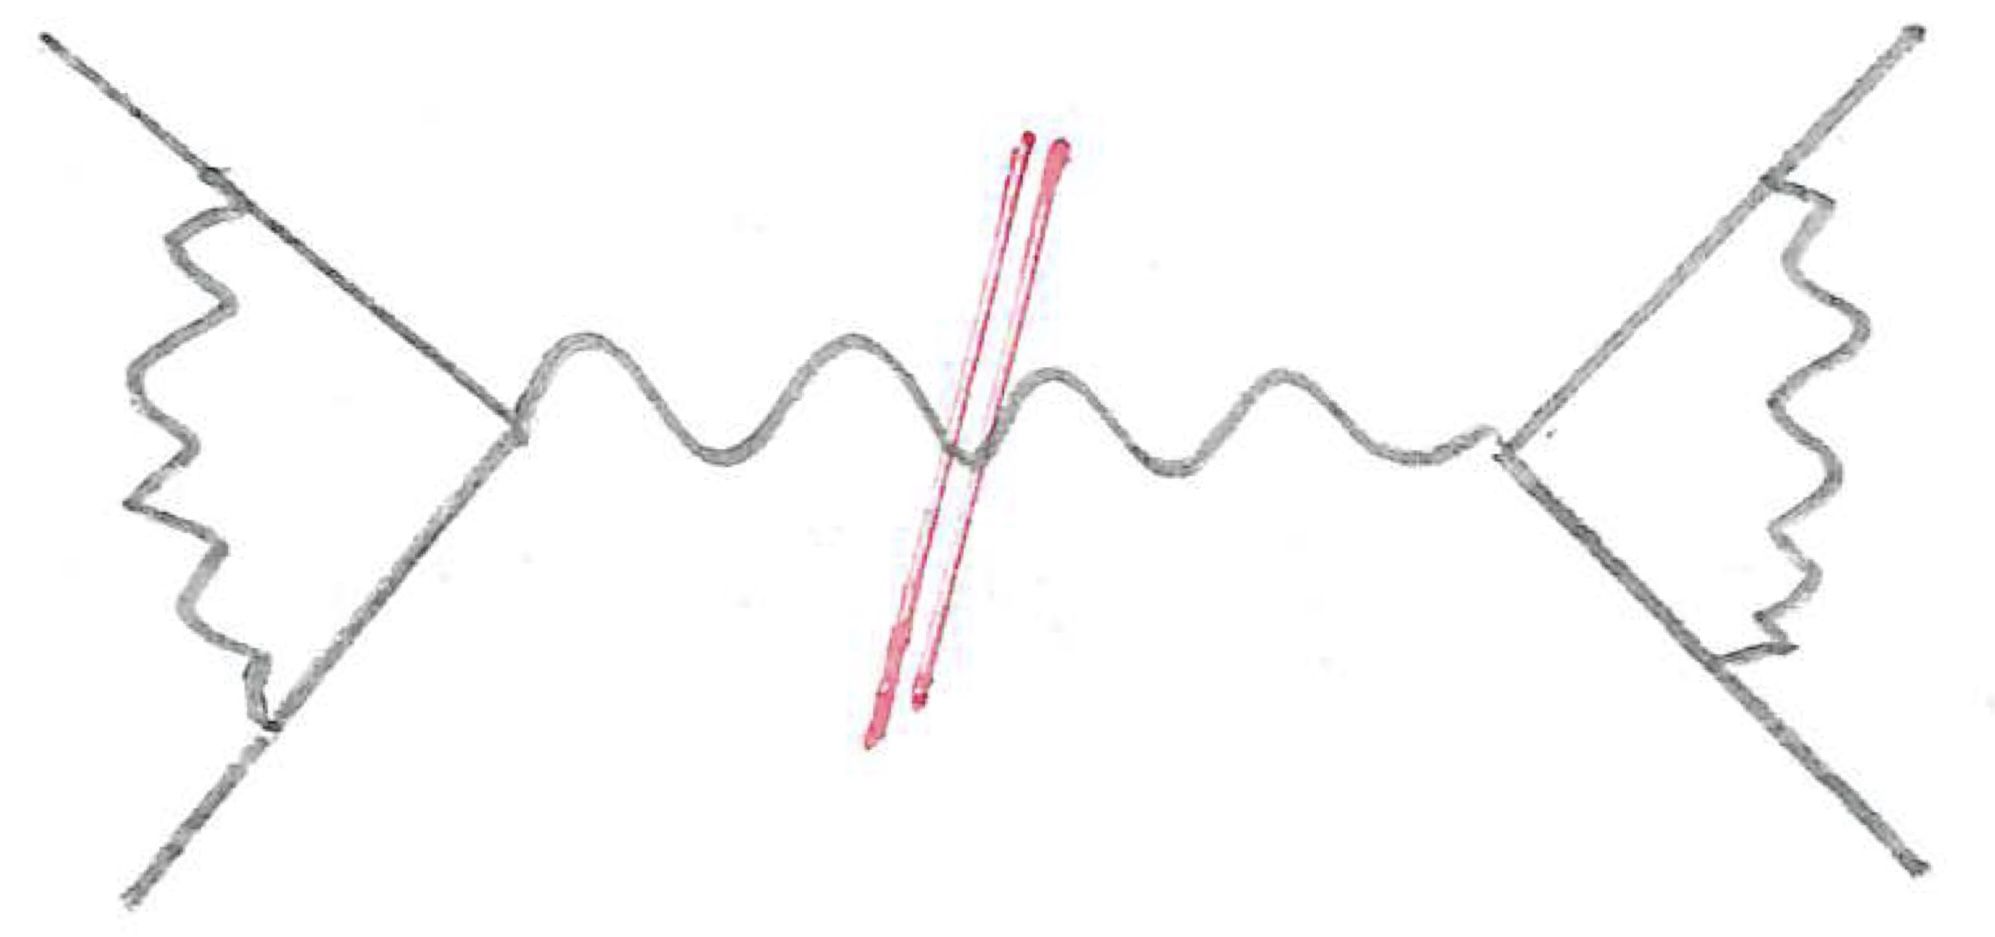
\includegraphics[]{images/QED_non1PI.jpg}}
\begin{definition}
    \textbf{(Diagramma Connesso.)}\\
    Un diagramma si dice \textbf{Connesso} quando è possibile trovare un percorso da un elemento all'altro senza ricorrere a salti.
    \label{def:connected_diagram}
\end{definition}
\begin{definition}
    \textbf{(Diagramma One-Particle Irreducible.)}\\
    Un diagramma si dice "one-Particle Irreducible" (\textbf{1PI}) quando non è possibile dividerlo in due tagliando un singolo propagatore.
    \label{def:1PI}
\end{definition}

\underline{\textbf{Notiamo}} come non ci sia perdita di generalità nel limitarsi allo studio di diagrammi connessi e 1PI, in quanto diagrammi disconnessi sono composizione di diagrammi connessi e diagrammi non-1PI sono ottenuti "incollando" insieme diagrammi 1PI.\\
In sostanza questa tipologia di diagrammi sono i building blocks di tutti i diagrammi più complessi.

Consideriamo allora un diagramma di QED generico, \textbf{connesso} e \textbf{1PI}, come quello riportato a lato. \marginnote{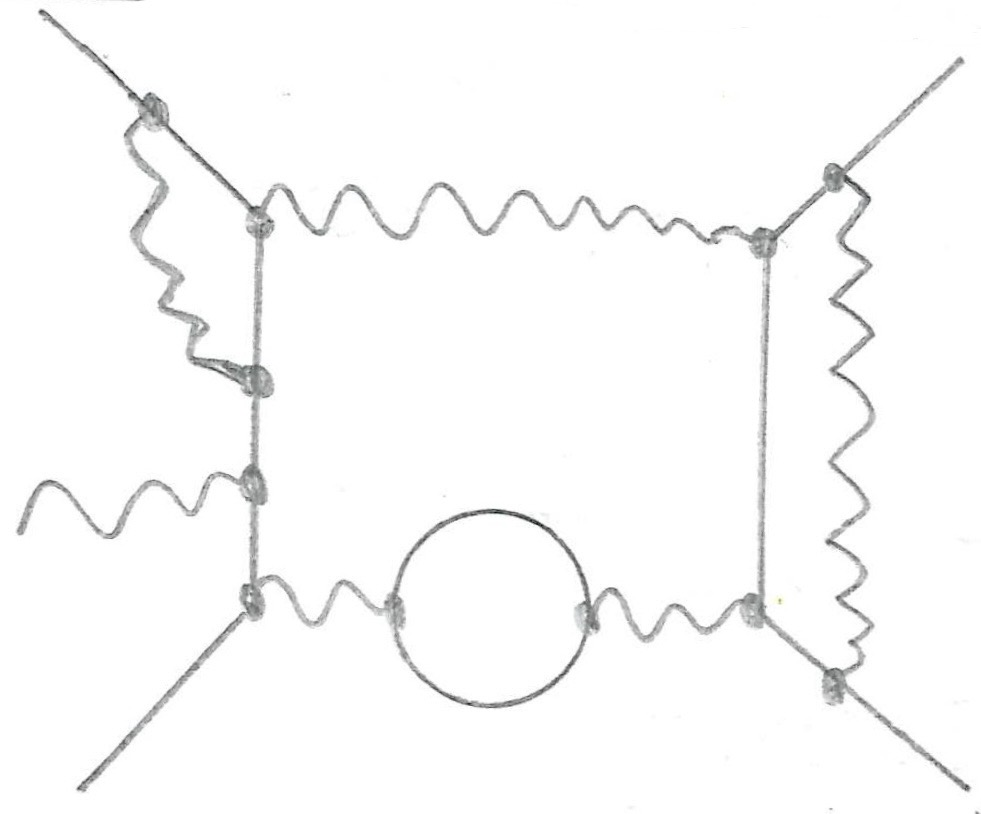
\includegraphics[]{images/QED_generic_1PI.jpg}}
Ci aspettiamo allora
\[
    \text{Diagramma} \sim \int\mathrm{\frac{d^4k_1 \cdot\cdot\cdot d^4k_L}{(\slashed k_i-m)\cdot\cdot\cdot k_j^2k_m^2}}
\]

dove i $\mathrm{k_i}$ sono generici 4-impulsi di loop sui quali stiamo integrando, con $\mathrm{i\in [1,L]}$ ed L numero di loop nel diagramma.

Contando le potenze dei 4-impulsi al numeratore e al denominatore, possiamo introdurre un concetto chiave, che guiderà il nostro studio della teoria della rinormalizzazione: il \textbf{Grado di Divergenza Superficiale}.
\begin{definition}
    \textbf{(Grado di Divergenza Superficiale.)}
    \begin{center}
    $\mathbf{D}\equiv$ potenza totale dei $\mathrm{k}$ nel numeratore $-$ potenza totale dei $\mathrm{k}$ nel denominatore.
    \end{center}
    \label{def:DoD_concept}
\end{definition}
Questa quantità dovrebbe darci un'idea del grado di divergenza dell'integrale, in quanto da un diagramma con grado di divergenza $\mathbf{D}$ ci aspettiamo un integrale del tipo:

    \[\int^\Lambda\mathrm{k^{D-1}\,d^4k} \Rightarrow \begin{cases}
    \text{power-divergent in $\Lambda$ se } D>0\\
    \text{log-divergent in $\Lambda$ se } D=0\\
    \text{convergente se } D<0
    \end{cases}\]


dove abbiamo introdotto un cutoff esplicito $\Lambda$ nell'estremo superiore dell'integrazione. 

\underline{\textbf{Nota:}} In questo momento siamo interessati al caso in cui $\mathrm{k}\rightarrow\infty$, a cui spesso ci si riferisce come "regione ultravioletta" (grande k implica piccole lunghezze d'onda) e di conseguenza, in caso di divergenza dell'integrale, si parla di \textbf{divergenza ultravioletta} (UV)\footnote{esiste anche quella infrarossa (IR)}.

\subsection{Formalizzazione di D in QED}
L'idea è quella di ridefinire il grado di divergenza sulla base delle caratteristiche del diagramma considerato. Per fare ciò definiamo le seguenti quantità:
\begin{center}
    \begin{tabular}{|c||l}
    \hline
      $N_e$        &  numero di gambe esterne "elettroniche"\\
      $N_\gamma$   &  numero di gambe esterne fotoniche\\
      $P_e$        &  numero di propagatori "elettronici"\\
      $P_\gamma$   &  numero di propagatori fotonici\\
      $V$          &  numero di vertici\\
      $L$          &  numero di loops \\
    \hline
    \end{tabular}
\end{center}

Notiamo ora come:
\begin{itemize}
    \item il propagatore fermionico sia della forma $\frac{i\mathrm{(\slashed k_i-m)}}{\mathrm{k_i^2-m^2}+i\epsilon}$, quindi $D=-1$. Possiamo allora dire che il contributo di $P_e$ contribuisce a D come $-P_e$;
    \item allo stesso modo il propagatore fotonico in gauge di Feyman si scrive $-\frac{ig^{\mu\nu}}{\mathrm{k^2}+i\epsilon}$, quindi $D=-2$ e $P_\gamma$ contribuisce come $-2P_\gamma$;
    \item non c'è dipendenza dall'impulso nel vertice di QED;
    \item ogni loop porta 4 potenze di k.
\end{itemize}

In conclusione si può scrivere:
\begin{equation}
    D = 4L - P_e - 2P_\gamma
    \label{eq:D_loop_propagators}
\end{equation}

Questa espressione può essere migliorata ancora di più se si lavora sul numero dei loops, che può essere definito come il numero di impulsi interni che non sono fissati da leggi di conservazione ad ogni vertice di interazione.

Diagrammi come quello del BhaBha scattering hanno L=0, in quanto l'impulso del propagatore è determinato dagli impulsi esterni, quindi non serve integrare.
\begin{example}
Prendiamo un diagramma come quello a destra, \marginnote{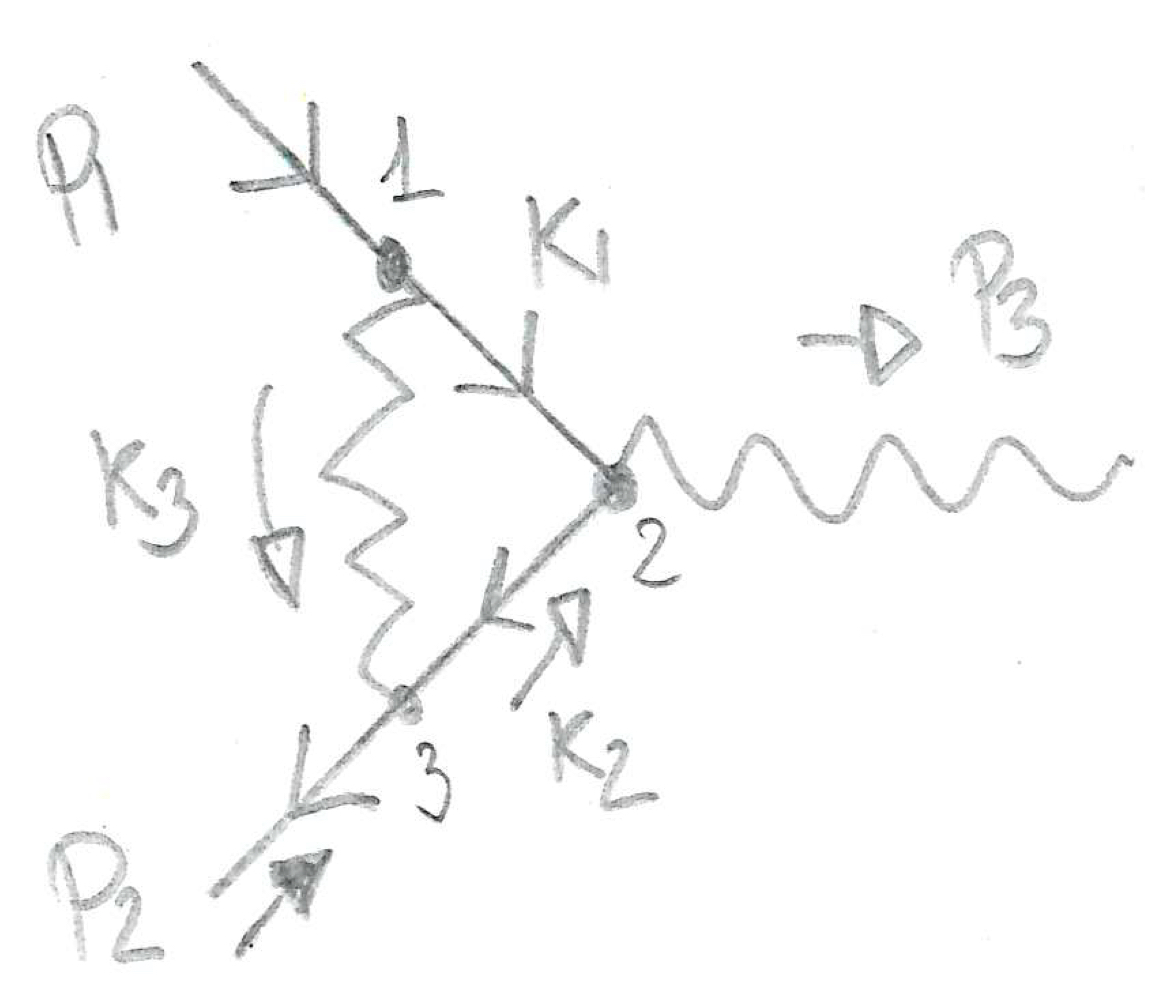
\includegraphics[]{images/QED_1Loop.jpeg}}siamo di fronte a 3 impulsi interni e 3 vertici, a cui corrispondono 3 leggi di conservazione.\\
Tuttavia, risolvendo il sistema ci accorgiamo che una delle 3 leggi non è altro se non la conservazione degli impulsi esterni e quindi non va a fissare alcun impulso interno.

Possiamo quindi esprimere due degli impulsi interni in funzione del terzo, quello su cui integriamo, quindi L=1 ed infatti abbiamo un loop!
\end{example}

Formalmente possiamo scrivere:
\begin{equation}
    L = P_e+P_\gamma - (V-1)
    \label{eq:L_propagators_vertices}
\end{equation}
dove riconosciamo il numero di impulsi interni, uno per propagatore, ed il numero di vincoli dalle leggi di conservazione (V-1).

Andiamo ora ad esplicitare il numero dei vertici nel diagramma, considerando prima di tutto un semplice vertice di QED ($ee\gamma$).\marginnote{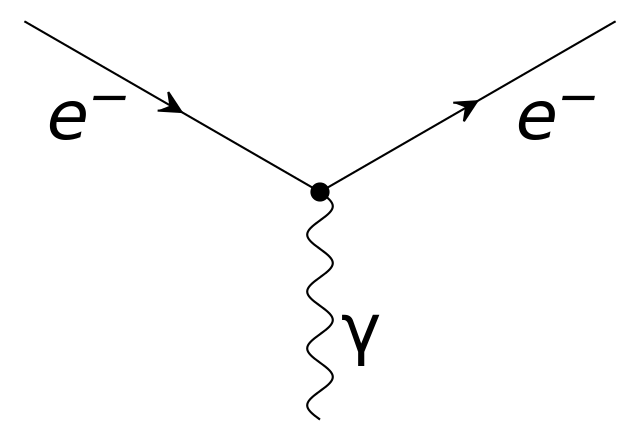
\includegraphics[]{images/QED_vertex.png}} È evidente il fatto che per V=N avremo 2V linee elettroniche ed V linee fotoniche.

A questo punto abbiamo due casistiche:
\begin{enumerate}
    \item per un diagramma con $N_\gamma$ linee esterne fotoniche, le rimanenti linee fotoniche saranno chiuse in propagatori, ed ogni propagatore chiude due linee $V - N_\gamma = 2P_\gamma$ ;
    \item per un diagramma con $N_e$ linee esterne elettroniche, con lo stesso ragionamento otteniamo $2V - N_e = 2P_e$ ;
\end{enumerate}

Ribaltando le equazioni troviamo quindi:
\begin{equation}
    \begin{cases}
        P_\gamma = \frac{1}{2}(V - N_\gamma) \\
        P_e = V - \frac{1}{2}N_e
    \end{cases}
    \label{eq:propagators}
\end{equation}

\marginnote{\begin{example}
    Un esempio di applicazione delle \ref{eq:propagators} è il seguente:
    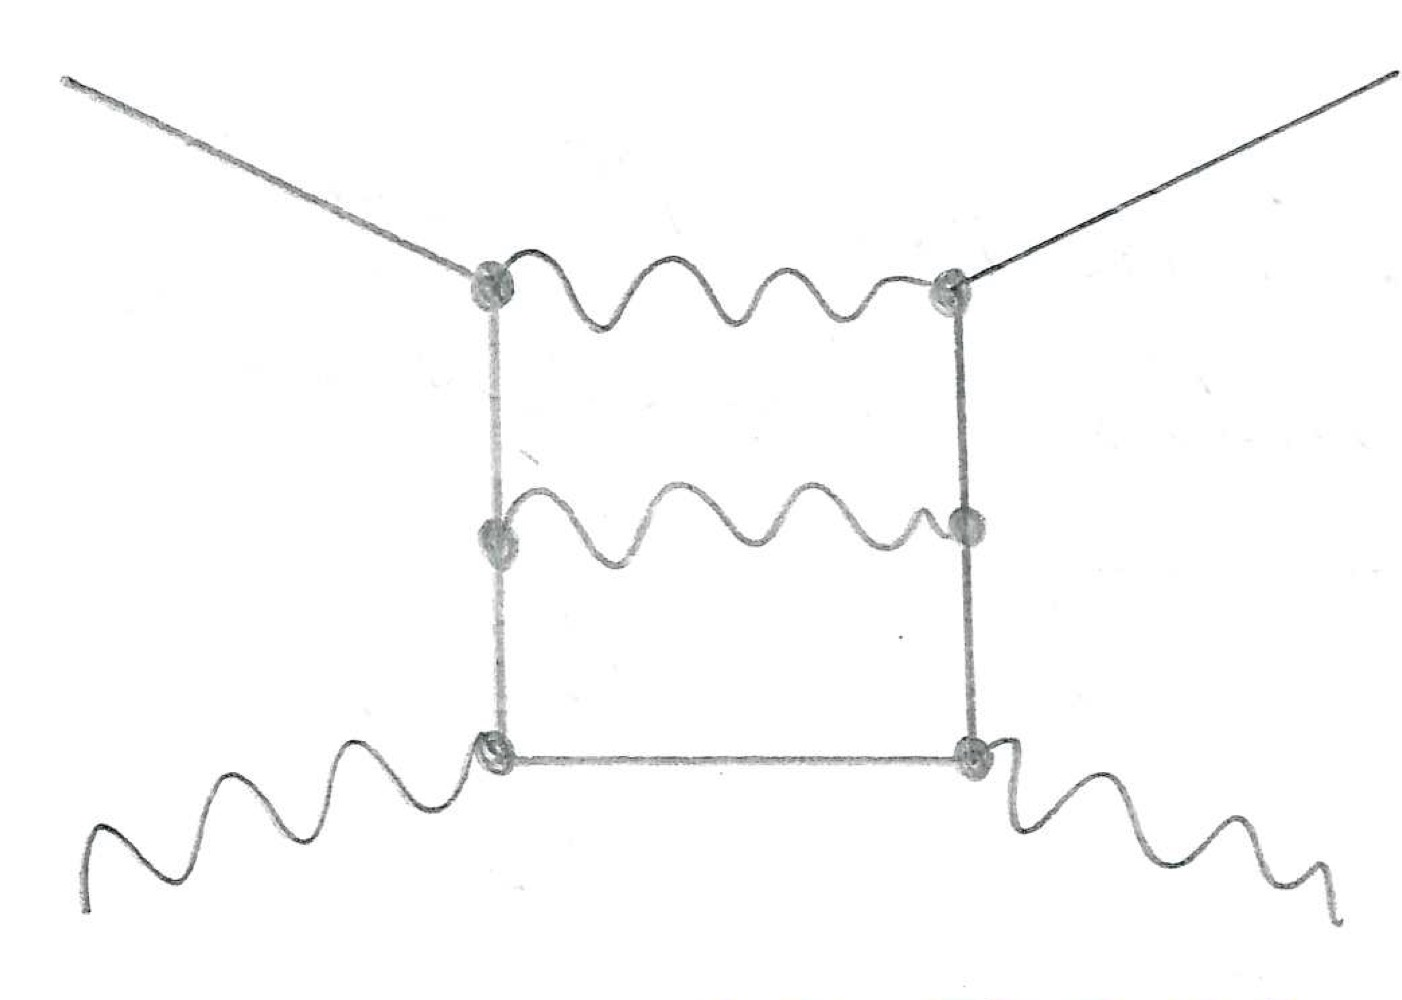
\includegraphics[]{images/QED_6vertex.JPG}\\
    $V=6, N_e=2, N_\gamma=2 \\ \Rightarrow P_\gamma=2, P_e=5$ 
    \label{ex:prop_eq_applic}
\end{example}}

Il gioco è fatto, combinando l'eq \ref{eq:propagators} e l'eq \ref{eq:L_propagators_vertices} possiamo riscrivere il numero dei loop in funzione di vertici e gambe esterne del diagramma:
\begin{equation}
    L = \frac{1}{2}(V-N_e-N_\gamma)+1
    \label{eq:L_extlegs_vertices}
\end{equation}

e sostituendo le equazioni \ref{eq:propagators}, \ref{eq:L_extlegs_vertices} nella \ref{eq:D_loop_propagators} abbiamo l'espressione che cercavamo, dipendente solo dalle gambe esterne del diagramma:

\begin{definition}
\textbf{(Grado di divergenza superficiale in QED, dimensione dello spazio-tempo d=4.)}
\begin{equation}
    D=4-\frac{3}{2}N_e-N_\gamma
    \label{eq:DoD_QED_4d}
\end{equation}
\label{def:DoD_ext_legs}
\end{definition}

\subsection{Teorie rinormalizzabili}
\marginnote{
\begin{tabular}{c|c|c|c|}
    \multicolumn{1}{c}{$\frac{\mathbf{N_e}\rightarrow}{\mathbf{N_\gamma}\downarrow}$} & \multicolumn{1}{c}{0} & \multicolumn{1}{c}{2} & \multicolumn{1}{c}{4}  \tabularnewline \hhline{~|*{3}{-}}
             0           &  4\cellcolor{red!25}  & 1 \cellcolor{red!25}  &   -2\cellcolor{blue!25}  \tabularnewline \hhline{~|*{3}{-}}
             1           &  3\cellcolor{red!25}  & 0 \cellcolor{red!25}   &   -3\cellcolor{blue!25}  \tabularnewline \hhline{~|*{3}{-}}
             2           &  2\cellcolor{red!25}    & -1\cellcolor{blue!25}  &  -4\cellcolor{blue!25}   \tabularnewline \hhline{~|*{3}{-}}
             3           &  1\cellcolor{red!25}    & -2\cellcolor{blue!25}  &  -5\cellcolor{blue!25}   \tabularnewline \hhline{~|*{3}{-}}
             4           &  0\cellcolor{red!25}    & -3\cellcolor{blue!25}  &  -6\cellcolor{blue!25}   \tabularnewline \hhline{~|*{3}{-}}
\end{tabular}
}
Abbiamo visto che guardando solo le gambe esterne dei diagrammi è possibile determinare il loro grado di divergenza superficiale e quindi classificarli: a lato è riportato il grado di divergenza al variare del numero di linee esterne fermioniche/fotoniche. In rosso le combinazioni che portano alla divergenza, in blu quelle che portano alla convergenza.

È evidente come il numero di ampiezze superficialmente divergenti sia finito. Parliamo di ampiezze invece di diagrammi in quanto il grado di divergenza (e quindi il numero di gambe esterne) identifica "categorie" contenti differenti tipologie di diagrammi (potenzialmente infiniti).

\begin{definition}
    \textbf{(Power-Counting Renormalizable Theory.)}\\ Una teoria si definisce rinormalizzabile per power-counting se il numero di ampiezze superficialmente divergenti è finito.
    \label{def:renormalizable_pc}
\end{definition}

Secondo la definizione \ref{def:renormalizable_pc}, la QED in d=4 dimensioni spazio temporali è rinormalizzabile per power-counting.

\section{Classificazione delle ampiezze divergenti}
Nel momento in cui consideriamo una teoria rinormalizzabile, abbiamo un numero finito di ampiezze superficialmente\footnote{a breve il termine "superficialmente" sarà abbandonato.} divergenti e la cosa interessante è che possiamo dividerle in tre gruppi, di cui si riportano alcuni esempi: 
\begin{enumerate}
    \item[i.] \textbf{Ampiezze realmente divergenti.}\\                
                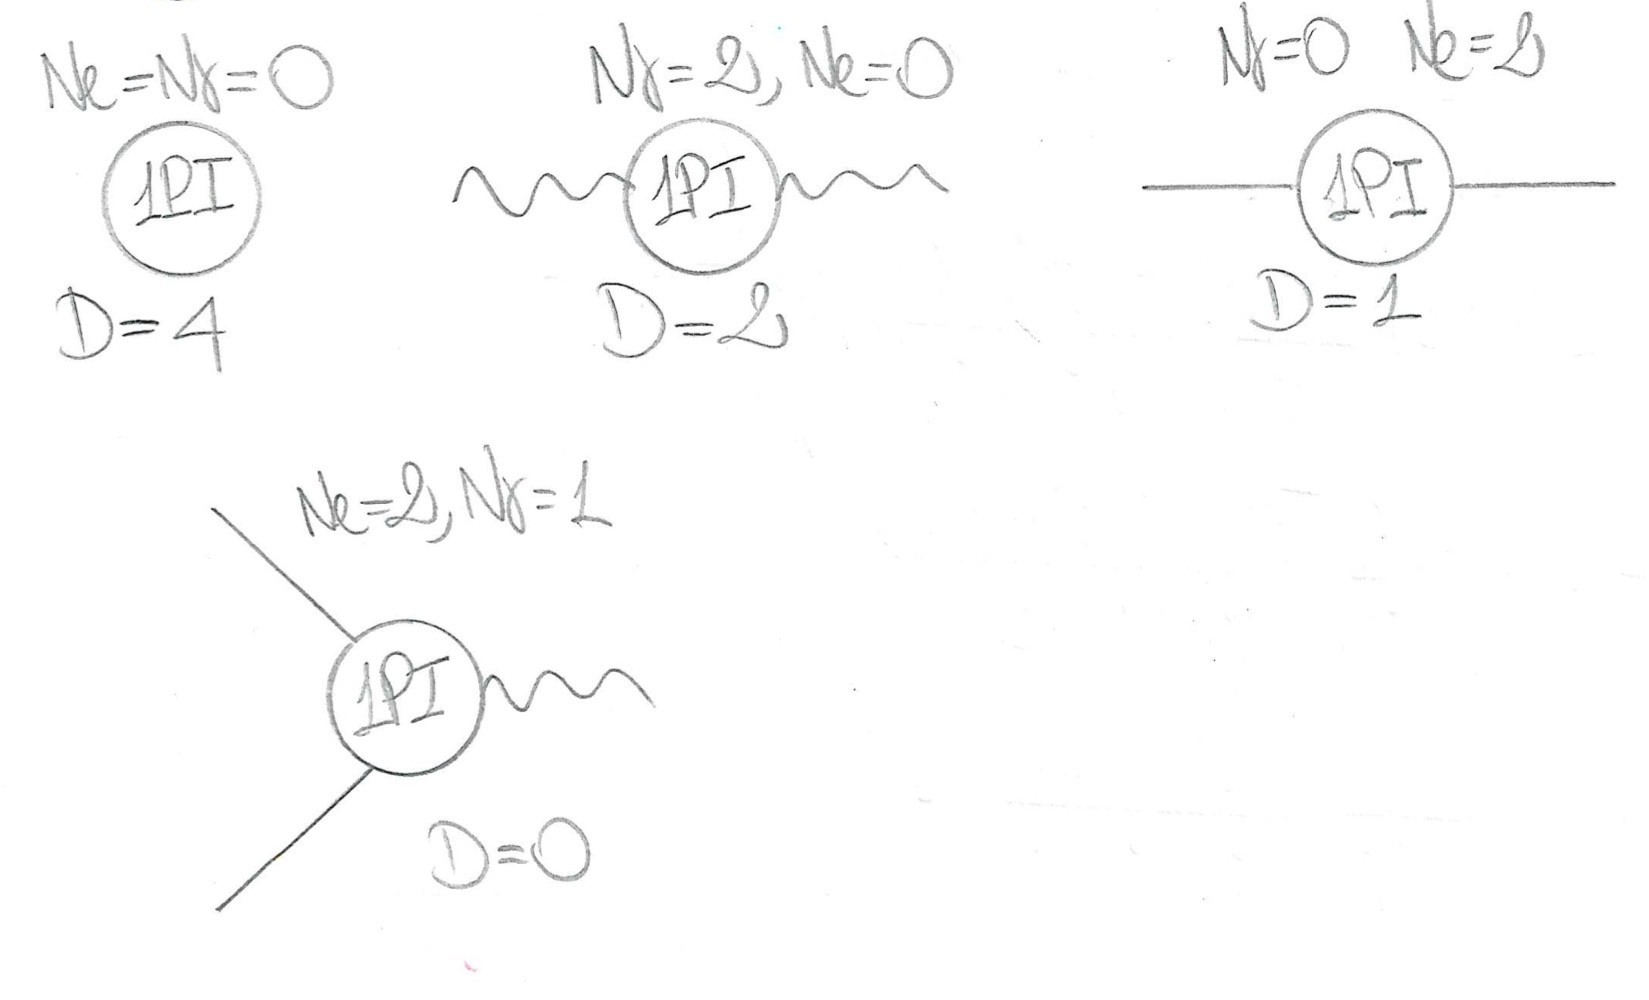
\includegraphics[]{images/Ampiezze_tipo1.jpg}
    \item[ii.] \textbf{Ampiezze divergenti superficialmente che vanno a zero ad ogni ordine.}\\
                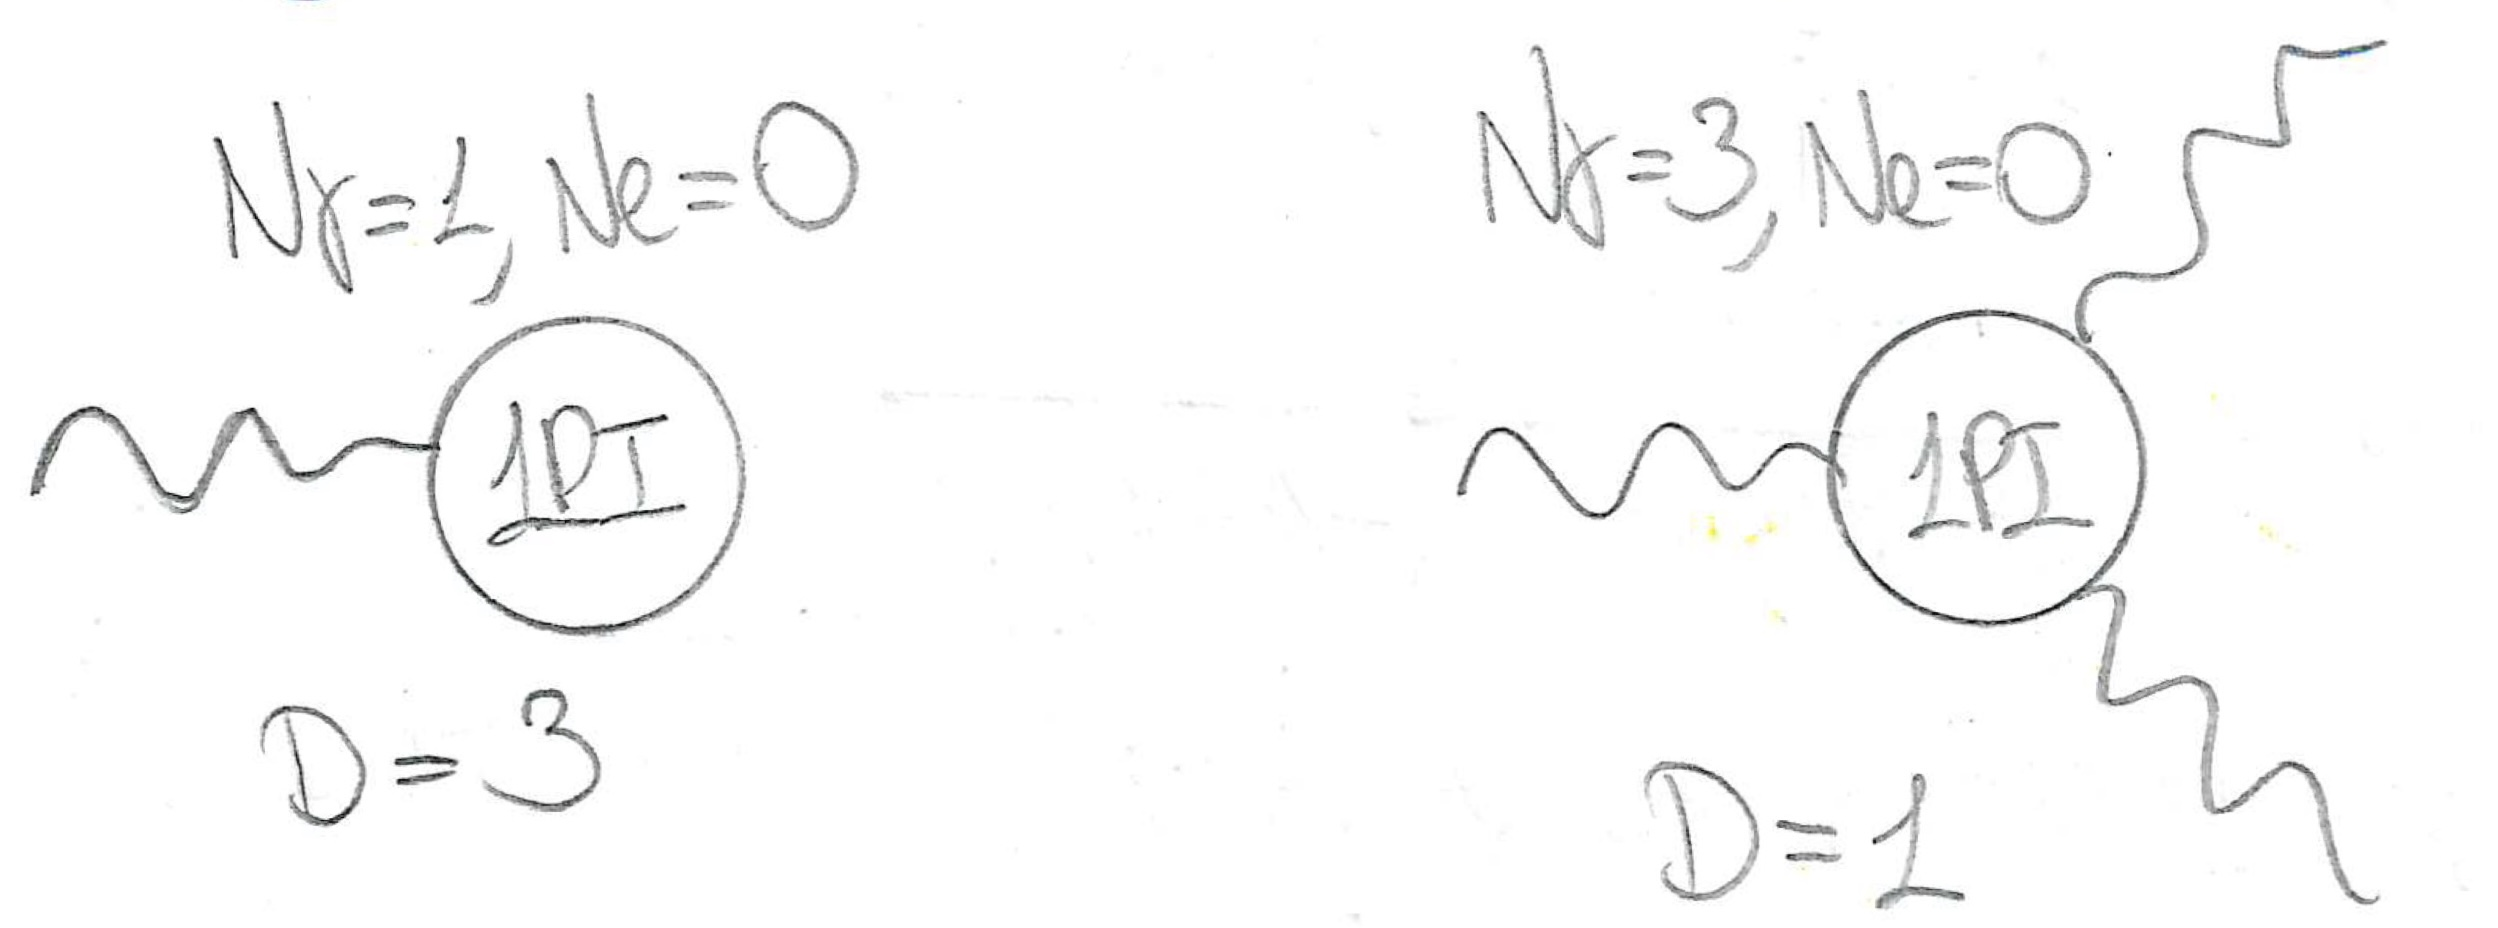
\includegraphics[]{images/Ampiezze_tipo2.jpg}\\
                \begin{exercise}
                Verificare tramite calcolo esplicito che due diagrammi appartenenti a questa categoria sono effettivamente nulli. \textbf{[svolti Lezione 1 p.12-15]}
                \end{exercise}
                Da questa categoria di ampiezze emerge un importante risultato, racchiuso nel teorema di Furry.
                \begin{theorem}
                \textbf{(Teorema di Furry.)}\\
                La funzione di correlazione associata ad un diagramma di Feynman composto da loop chiusi di linee fermioniche e da un numero dispari di fotoni esterni è sempre nulla in QED.
                \end{theorem}
                \underline{\textbf{Nota:}} Questo teorema è valido ad ogni ordine perturbativo, ed è una conseguenza dell'invarianza della QED sotto coniugazione di carica.
                
                \begin{proof}
                Lavoriamo sulla funzione di correlazione di un diagramma composto da n-fotoni:
                \[\langle\Omega|T[A^{\mu_1}(X_1)\cdot\cdot\cdot A^{\mu_n}(X_n)]|\Omega\rangle\]
                Sotto coniugazione di carica la corrente $\bar\Psi\gamma^\mu\Psi$ cambia segno, di conseguenza, per mantenere l'interazione $A_\mu\bar\Psi\gamma^\mu\Psi$ invariata, anche $A^\mu$ deve cambiare di segno sotto coniugazione di carica, in formule:
                
                \[\mathbb{C}^{-1} (\bar\Psi\gamma^\mu\Psi) \mathbb{C} = - \bar\Psi\gamma^\mu\Psi\]
                \[
                \mathbb{C}^{-1} A^\mu \mathbb{C} = - A^\mu
                \]

                Combinando quanto appena detto con la funzione di correlazione, sfruttando il fatto che possiamo inserire $\mathbb{C}\mathbb{C}^{-1}=\mathbb{1}$ a piacimento, così come la possibilità di portare dentro e fuori dal T-ordering l'operatore $\mathbb{C}$ ed il fatto che il vuoto $\Omega\rangle$ è invariante sotto coniugazione di carica e può quindi assorbire gli operatori esterni in eccesso, alla fine si ottiene:
                \[\langle\Omega|T[A^{\mu_1}(X_1)\cdot\cdot\cdot A^{\mu_n}(X_n)]|\Omega\rangle = (-1)^n\langle\Omega|T[A^{\mu_1}(X_1)\cdot\cdot\cdot A^{\mu_n}(X_n)]|\Omega\rangle
                \]
                È quindi evidente che, per n dispari, tale funzione di correlazione vada necessariamente a zero.
                \end{proof}
                \marginnote{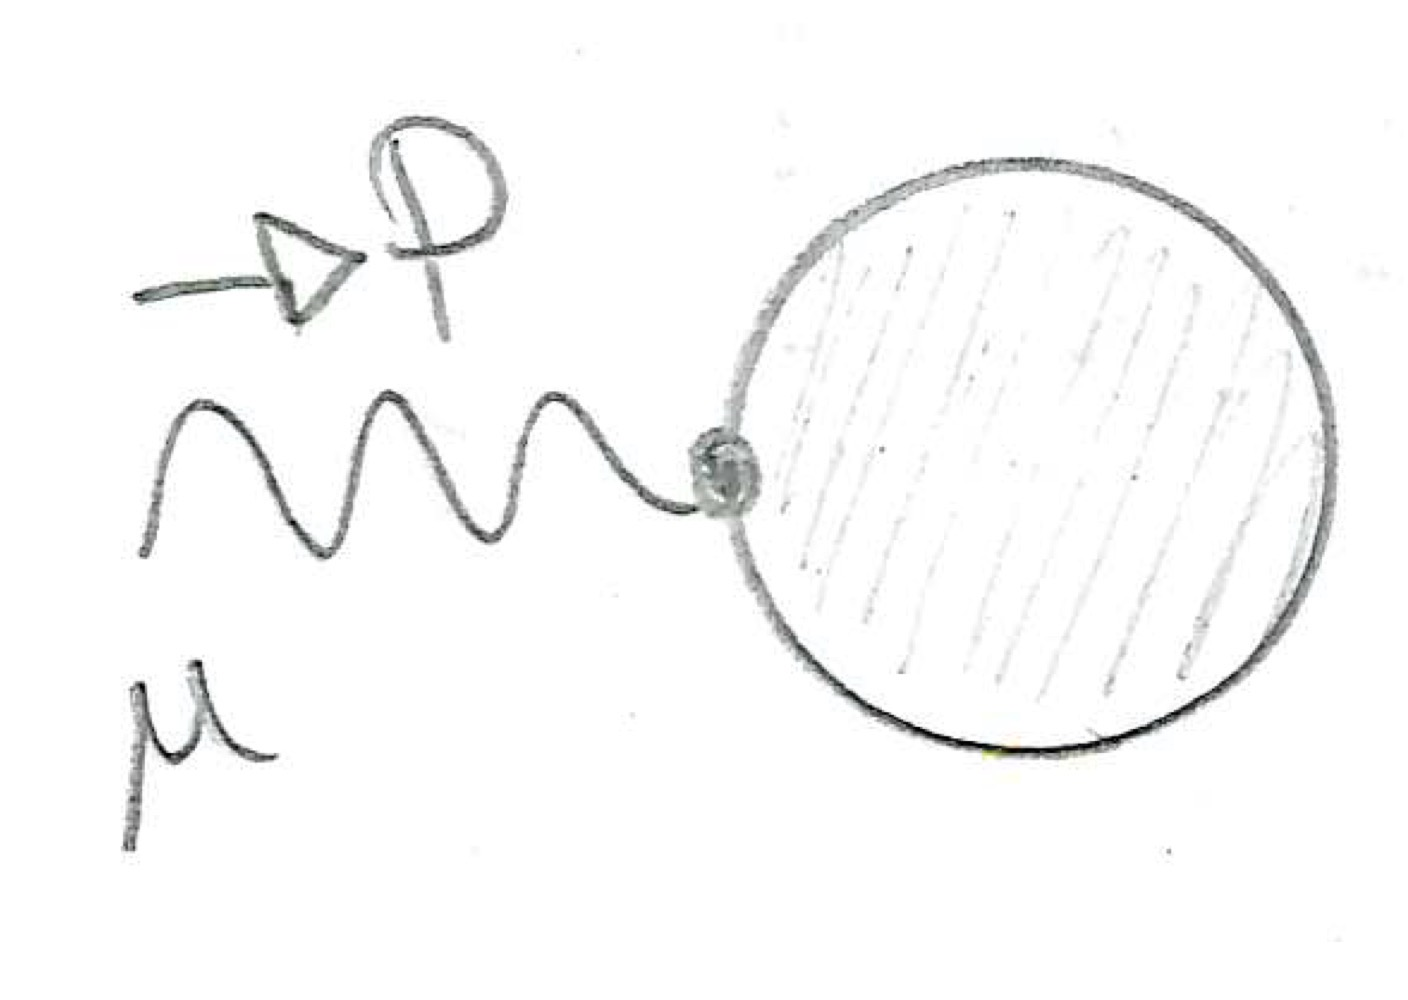
\includegraphics[]{images/tadpole_diagram.jpg}\\ Diagramma girino discusso nella Nota \ref{note:tadpole}}
                \begin{nota}
                Se consideriamo il diagramma con $N_\gamma=1, N_e=0$ (in gergo questa tipologia di diagrammi si chiama "girino"), anche se per assurdo non sussistesse la simmetria sotto coniugazione di carica in QED, questo diagramma andrebbe a zero ugualmente per via dell'invarianza sotto trasformazione di Lorentz.

                L'elemento di matrice associato sarà infatti \[i\mathscr{M}^\mu \simeq p^\mu f(p^2)\]ma la conservazione dell'impulso richiede che p=0, non essendoci alcun impulso uscente.

                Di conseguenza l'ampiezza del diagramma ad un fotone è nulla.\\
                
                Questo esempio è istruttivo in quanto dimostra come il grado di divergenza superficiale non sia in grado di "vedere le simmetrie della teoria".
                \label{note:tadpole}
                \end{nota}
            

    \item[iii.] \textbf{Ampiezze divergenti superficialmente che in realtà convergono.}\\ 
                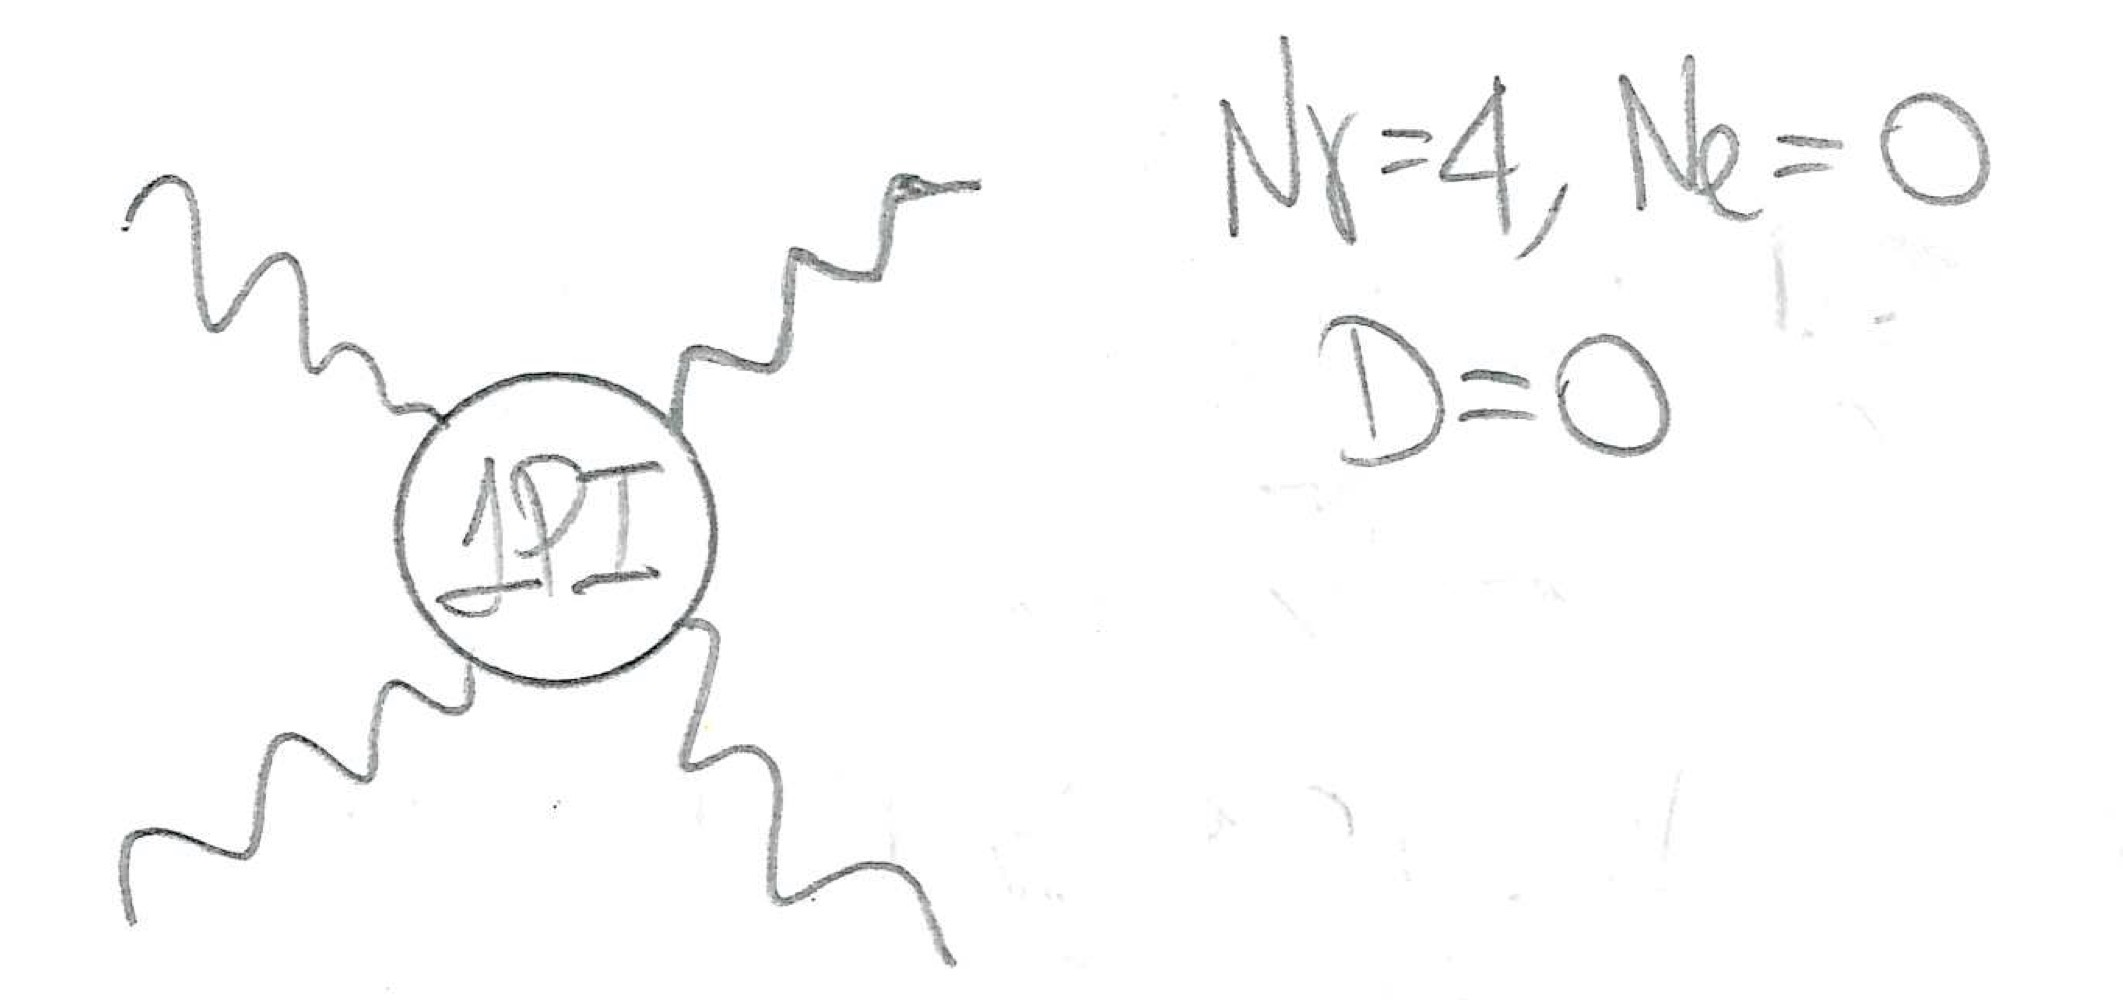
\includegraphics[]{images/Ampiezze_tipo3.jpg}\\
                \begin{exercise}
                    Considerare l'ampiezza con $N_\gamma = 4, N_e = 0$ e scrivere tutti i diagrammi che vi contribuiscono. Mostrare che l'ampiezza risulta nulla. \textbf{[conti svolti Lezione 2 p.20-25]}
                    \label{ex:4phot_ampl}
                \end{exercise}
                Al di là dei conti, proviamo a trovare una spiegazione più "intuitiva", possibilmente valida a tutti gli ordini. Per far ciò ci viene in aiuto una particolare proprietà del grado di divergenza.
                
                In generale l'ampiezza può dipendere anche dagli impulsi esterni, possibilmente fissati (ad esempio se si considera un particolare esperimento):
                \[
                i\mathscr{M}(p_i) \sim \int\mathrm{\frac{d^4k_1 \cdot\cdot\cdot d^4k_L}{k_1^2 \cdot\cdot\cdot [(k_i-p_i)^2-m^2] \cdot\cdot\cdot k_n^2}}
                \]
                a cui possiamo associare un grado di divergenza superficiale $D=4L-2n$.
                
                Se allora deriviamo rispetto $p_i$:
                \[
                i\frac{\partial\mathscr{M}}{\partial p_i^\mu}(p_i) \sim \int\mathrm{\frac{d^4k_1 \cdot\cdot\cdot d^4k_L}{k_1^2 \cdot\cdot\cdot [(k_i-p_i)^2-m^2]^2 \cdot\cdot\cdot k_n^2}(k_i-p_i)_\mu}
                \]
                è evidente come alla derivazione sia associata una riduzione del grado di divergenza superficiale: $D' = D - 1$.

                Possiamo quindi pensare di espandere l'ampiezza in serie di potenze intorno a $p_i=0$:
                \begin{equation}
                    \mathscr{M}(p_i) \approx \mathscr{M}(p_i=0) + \frac{\partial\mathscr{M}}{\partial p_i^\mu}p_i^\mu +\, \cdot\cdot\cdot
                    \label{eq:amplit_powerseries}
                \end{equation}
                L'osservazione che si può fare è che il primo termine (l'ampiezza con gli impulsi esterni posti a zero) è in grado di "catturare" il grado di divergenza dell'intera ampiezza, mentre ogni ordine successivo riduce D di 1 ogni volta. 

                Se \textbf{torniamo ora all'ampiezza a 4 fotoni} e applichiamo quanto appena trovato:\\
                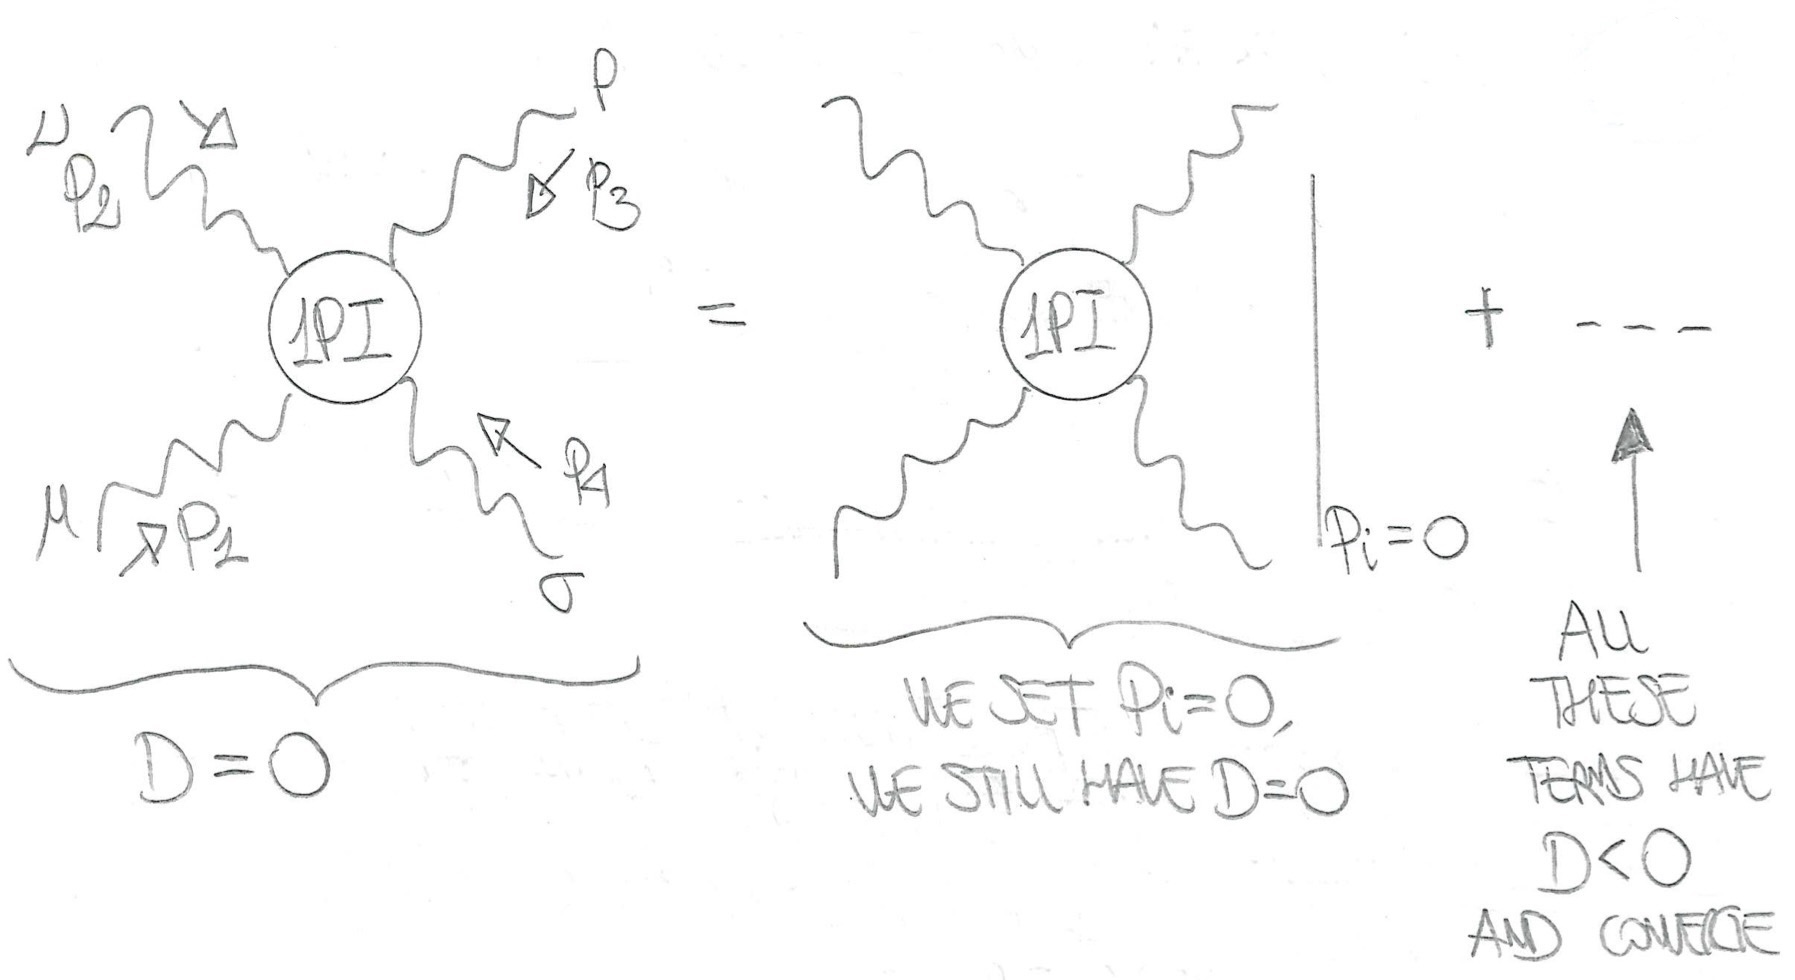
\includegraphics[]{images/4phot_expansion.jpg}\\
                che tradotto in equazioni ci dà la seguente struttura:
                \[
                \mathscr{M}^{\mu\nu\rho\sigma}(p_1,p_2,p_3,p_4) = \mathscr{M}^{\mu\nu\rho\sigma}_{UV}(p=0)+ \mathscr{M}^{\mu\nu\rho\sigma}_{\text{FINITE}}(p_1,p_2,p_3,p_4)
                \]
                abbiamo quindi isolato la componente divergente, che risulta essere un tensore. Tuttavia, dato che abbiamo posto i $p_i=0$, l'unico modo per parametrizzarlo è grazie al tensore metrico.

                Scriviamo allora:
                \begin{equation}
                \mathscr{M}^{\mu\nu\rho\sigma}_{UV}(p=0) = (g^{\mu\nu}g^{\rho\sigma} + g^{\mu\sigma}g^{\nu\rho} + g^{\mu\rho}g^{\nu\sigma})\times M_{UV}
                \label{eq:amplit_divergent_structure}
                \end{equation}
                dove $M_{UV}$ è un invariante di Lorentz \textbf{divergente}. Notiamo come questa espressione sia invariante sotto una generica permutazione degli indici, per via della simmetria di Bose.

                La cosa interessante a questo punto è che, invocando le \textbf{Identità di Ward-Takahashi}\footnote{che verranno trattate più formalmente in seguito}, si può mostrare che questa espressione si annulla.

                In particolare, nel caso puramente fotonico con $n$ linee esterne \marginnote{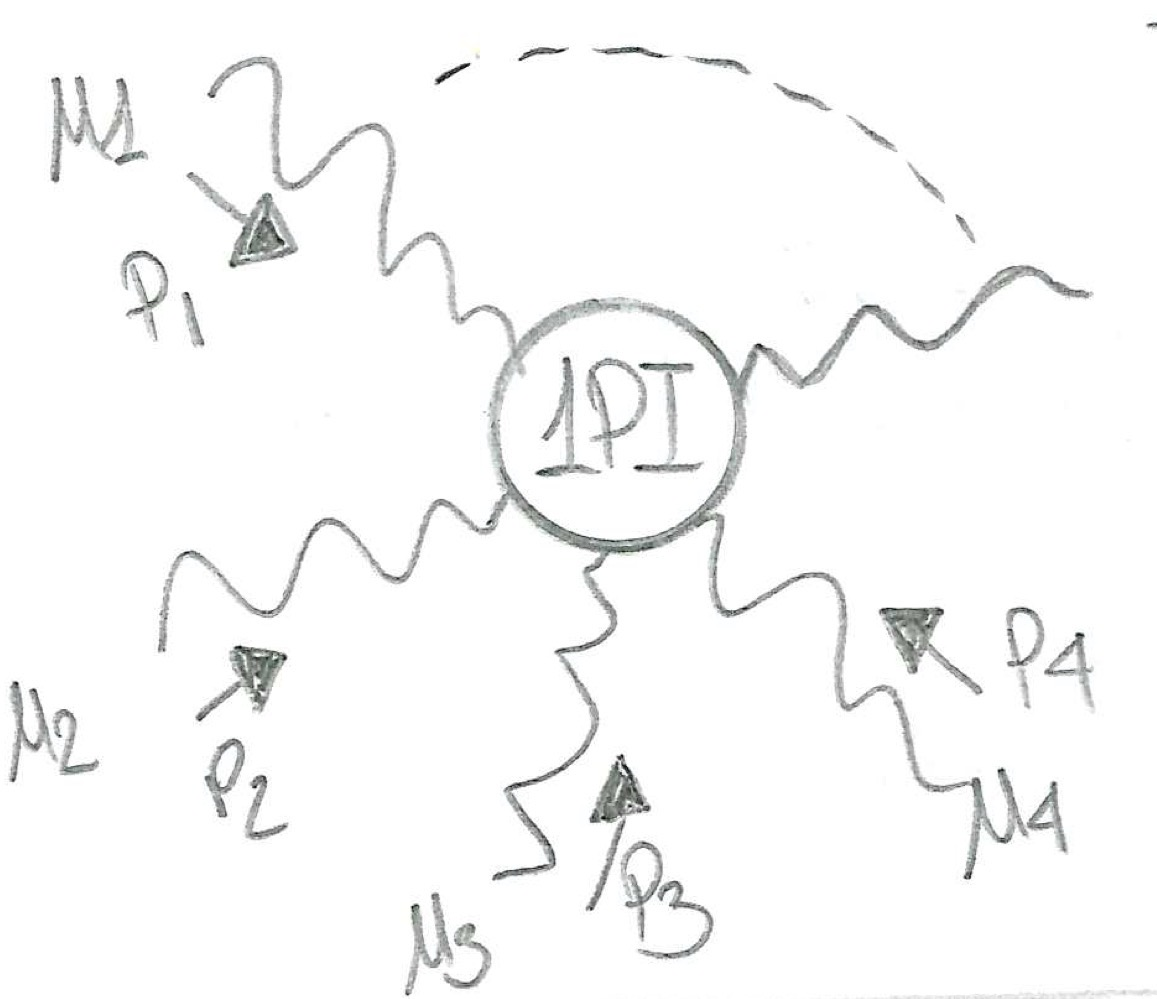
\includegraphics[]{images/Ampiezza_nphoton.jpg}}, a cui corrisponde la generica ampiezza
                \[
                i\mathscr{M}^{\mu_1,...,\mu_n}(p_1, ..., p_n)
                \]
                possiamo scrivere:
                \begin{theorem}
                    \textbf{(Identità di Ward-Takahashi, caso ad $n$ fotoni esterni.)}
                    
                    

                    Quando contraiamo l'indice di Lorentz $\mu_j$ di ogni fotone (nell'ampiezza) con il quadrimpulso $(p_j)_{\mu_j}$ dello stesso fotone dobbiamo ottenere come risultato zero.\\
                    In formule si traduce:
                    \[
                    (p_j)_{\mu_j}\mathscr{M}^{\mu_1,...,\mu_j,...\mu_n}(p_1, ..., p_n) = 0 \, \forall \, j=1,...,n
                    \]
                    \label{th:WTI_nphot}
                \end{theorem}
                \marginnote{Attenzione: in questo caso non è necessario che i fotoni siano tutti on-shell, difatti le identità di W-T si applicano alle funzioni di correlazione nello spazio dell'impulso. la situazione è diversa nel caso dell'{identità di Ward}, in cui la richiesta di particelle on-shell è necessaria.}
                
                \begin{nota}
                    Dal punto di vista fisico, quanto enunciato nel teorema \ref{th:WTI_nphot} è conseguenza dell'invarianza di gauge: il \href{https://physics.stackexchange.com/questions/231092/general-principles-require-that-a-massless-vector-couple-to-a-conserved-current}{fotone si accoppia con una corrente conservata}. Questo fatto genera una serie di relazioni di consistenza tra funzioni di correlazione che sono poi le identità di Ward-Takahashi, che volendo possono essere viste come l'\href{https://en.wikipedia.org/wiki/Ward%E2%80%93Takahashi_identity}{analogo quantistico della corrente conservata classica associata ad una simmetria continua per conseguenza del teorema di Noether}.
                    \label{note:WT_Gaugeiv_conseq}
                \end{nota}
                
                Tornando ora al nostro risultato, scriviamo:
                \[
                p_{1\,\mu}\mathscr{M}^{\mu\nu\rho\sigma}(p_{1,..,4}) = p_{1\,\mu}\mathscr{M}^{\mu\nu\rho\sigma}_{UV}(p_i=0) + p_{1\,\mu}\mathscr{M}^{\mu\nu\rho\sigma}_\text{FINITE}(p_{1,..,4}) \overset{!}{=} 0
                \]
                Ma siccome il termine finito non può cancellare quello UV-divergente, allora entrambi i termini devono essere nulli!

                Ricordando l'eq. (\ref{eq:amplit_divergent_structure}):
                
                \begin{equation}
                \begin{split}  
                p_{1\,\mu}
                &(g^{\mu\nu}g^{\rho\sigma} + g^{\mu\sigma}g^{\nu\rho} + g^{\mu\rho}g^{\nu\sigma})\times M_{UV} =\\
                &= (p_{1\,\nu}g^{\rho\sigma} + p_{1\,\sigma}g^{\nu\rho} + p_{1\,\rho}g^{\nu\sigma})\times M_{UV} \\
                &\Rightarrow \boxed{M_{UV}=0}
                \end{split}
                \label{eq:WTI_4phot_UV}
                \end{equation}
                
                Quello che ci dice l'eq. (\ref{eq:WTI_4phot_UV}) è che \textit{l'identità di W-T non consente la divergenza UV per l'ampiezza a 4 fotoni}.\\

                \textbf{Notiamo} inoltre che in generale $M_{UV}$ è una somma cumulativa di diagrammi fino a un certo ordine in teoria delle perturbazioni, quindi le identità di W-T ci dicono solo che la somma cumulativa dei diagrammi è libera dalla divergenza ultravioletta, \textbf{i singoli diagrammi che contribuiscono a tale somma possono divergere!}\footnote{come si può vedere svolgendo l'esercizio \ref{ex:4phot_ampl}} Questa è una proprietà del tutto generale delle identità di W-T.
\end{enumerate}
\section{Generalizzazione}
Abbiamo visto come il grado di divergenza superficiale $D$ sia uno strumento molto utile nel momento in cui si vuole organizzare le ampiezze UV-divergenti, tuttavia ci sono casi in cui fallisce.

In particolare:
\begin{itemize}
    \item per il caso dell'ampiezza a 3 fotoni $D=1$, tuttavia per ragioni di simmetria l'ampiezza va identicamente a zero.
    \item per il caso dell'ampiezza a 4 fotoni $D=0$, tuttavia a causa delle proprietà strutturali della teoria (ossia il fatto che gli infiniti si cancellano quando si considera la somma cumulativa dei diagrammi) anche qui l'ampiezza non diverge.
\end{itemize}

\marginnote{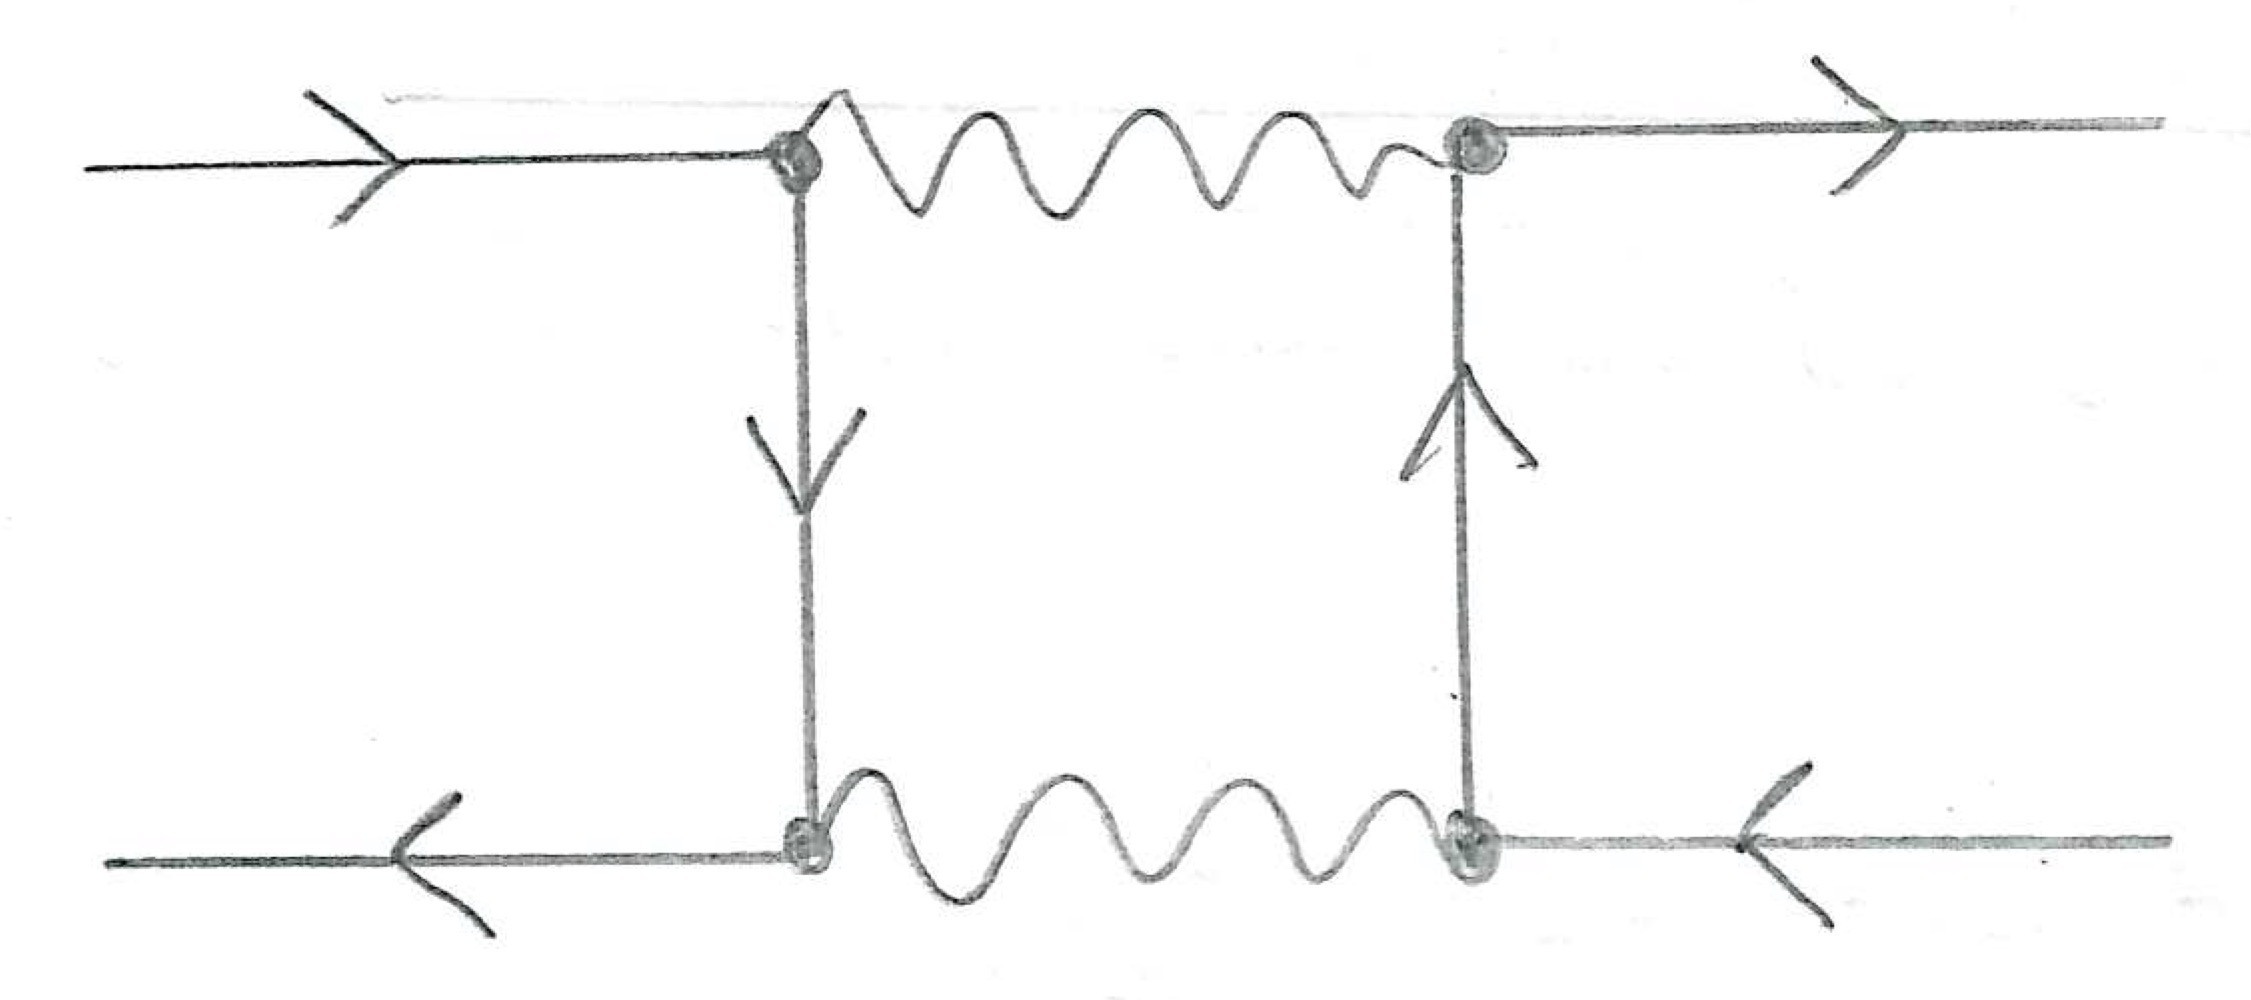
\includegraphics[]{images/4electr_1loop.jpg}\\
il diagramma con 4 linee fermioniche esterne ad un loop.\\ 
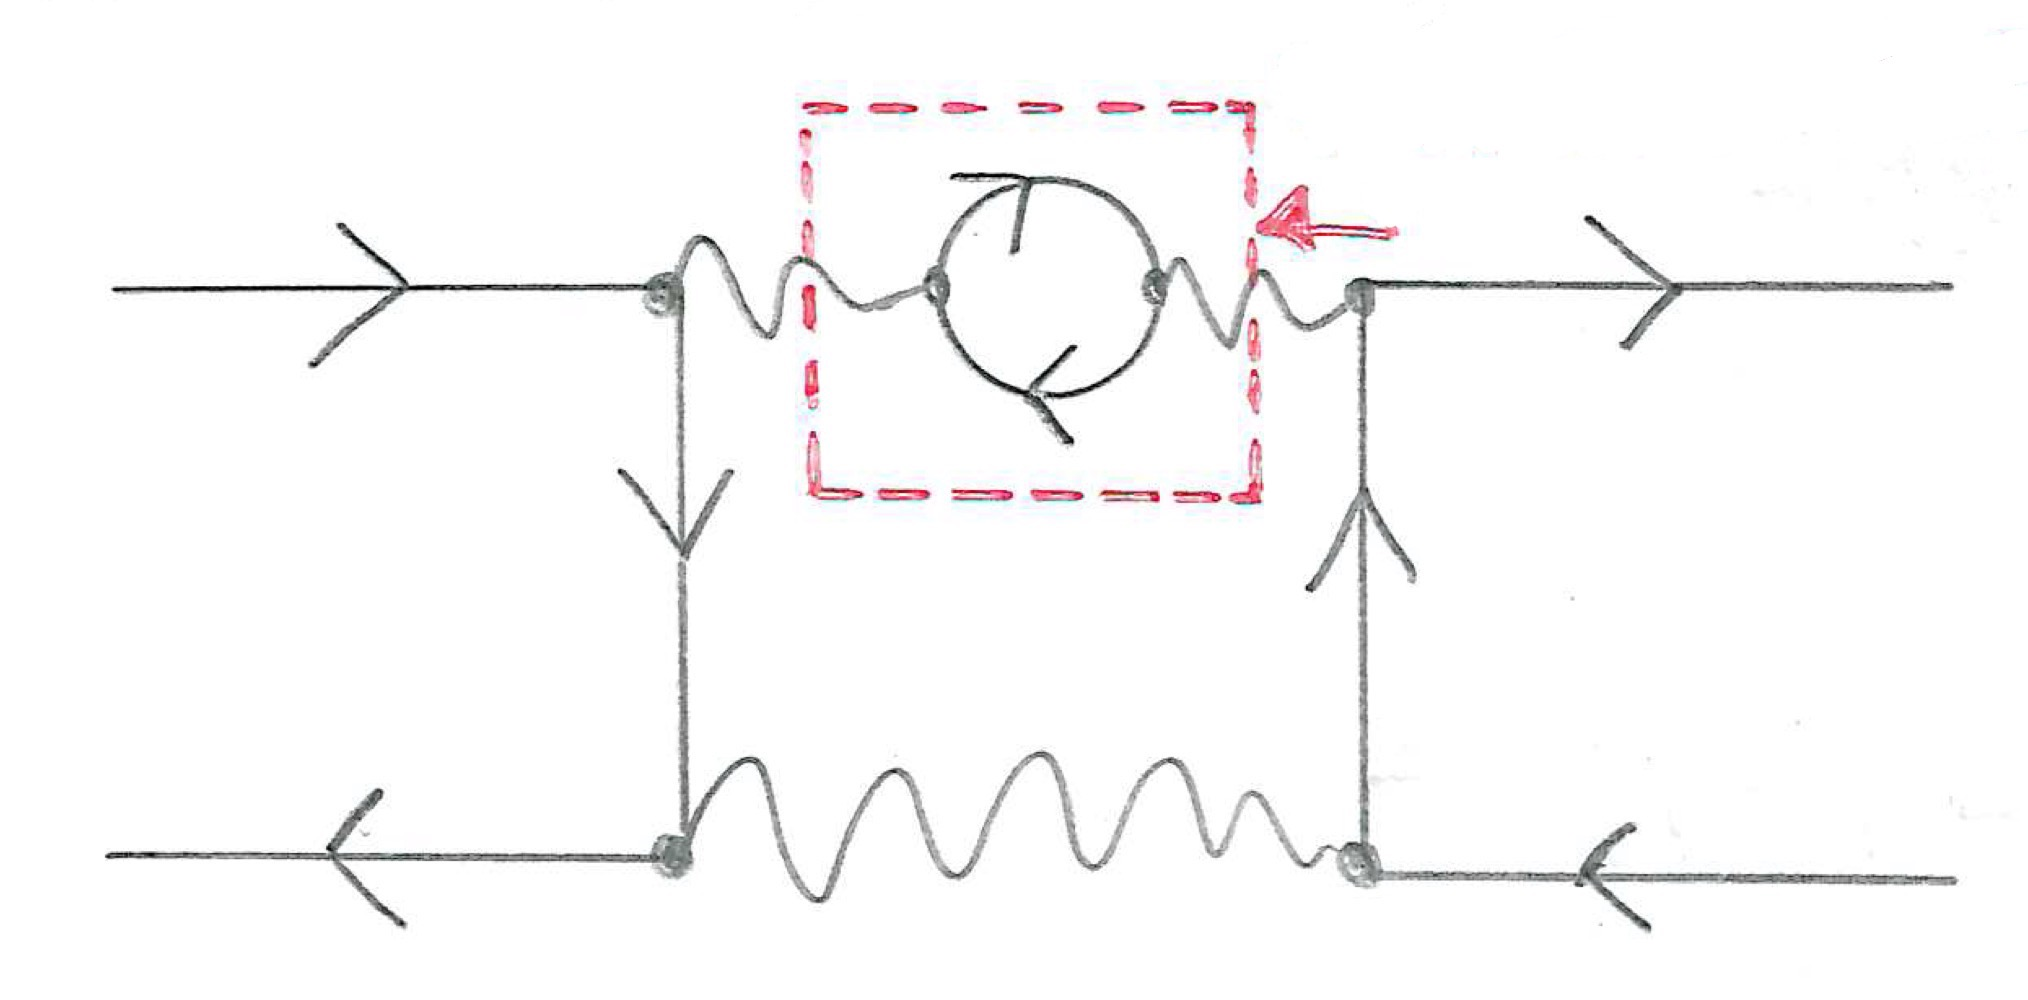
\includegraphics[]{images/4electr_2loop.jpg}\\ 
il diagramma con 4 linee fermioniche esterne a due loop.}
Un terzo caso che ancora non abbiamo trattato ci consente di fare un'ulteriore considerazione.

Consideriamo $N_e=4, N_\gamma=0$, allora $D=-2$ e il diagramma \textbf{dovrebbe} convergere.\\
\underline{A un loop} abbiamo un diagramma che effettivamente non diverge nel range UV.\\
\underline{A due loop}, però, ci ritroviamo con un \textcolor{red}{sotto-diagramma} che sappiamo essere divergente. Quindi, nonostante aggiungere vertici non modifichi $D$, il diagramma a due loop diverge lo stesso.

Ciò che è interessante notare è che \textbf{questo tipo di divergenza l'abbiamo già incontrata}, quindi se riusciamo a trovare il modo di eliminare la divergenza delle ampiezze "realmente divergenti", come quella nel sotto-diagramma, allora possiamo correggere anche il problema che sorge in questo caso!

Prima di lanciarci a capofitto nel calcolo di qualsivoglia diagramma, è opportuno discutere il modo in cui si arriva alla generalizzazione del grado di divergenza superficiale in più dimensioni dello spazio-tempo.

\subsection{QED in più dimensioni}
L'utilità di questa discussione è del tutto generale, lo faremo in termini di QED, ma risulta utile anche per la teoria della regolarizzazione (che vedremo in seguito), così come per altre teorie come quella della materia condensata o la teoria delle stringhe.

Considerando uno spazio-tempo di dimensione generica $\dim = \mathsf{d}$, abbiamo $\int d^4k \rightarrow \int d^\mathsf{d}k$ e di conseguenza $D(\dim = \mathsf{d}) = \mathsf{d}\cdot L - P_e - P_\gamma $, utilizzando la stessa notazione introdotta in precedenza.

Valgono ancora le relazioni:
\[
\begin{cases}
P_e = V - N_e\\
P_\gamma = \frac{1}{2}(V - N_\gamma)\\
L = \frac{1}{2}(V - N_e - N_\gamma) + 1
\end{cases}
\]

E con un esercizio di pura algebra si trova:
\begin{equation}
    D = \mathsf{d} + \bigg(\frac{\mathsf{d}-4}{2}\bigg)V - \bigg(\frac{\mathsf{d}-1}{2}\bigg)N_e - \bigg(\frac{\mathsf{d}-2}{2}\bigg)N_\gamma
    \label{eq:generalized_degree_divergence}
\end{equation}

È evidente come ora $D$ dipenda dal numero dei vertici!\\

Analizziamo i casi possibili:
\begin{itemize}
    \item $\mathbf{\mathsf{d} = 4}$\\
          È il caso trattato in precedenza, la dipendenza dai vertici scompare e abbiamo una teoria rinormalizzabile.
    \item $\mathbf{\mathsf{d} < 4}$\\
          Il coefficiente $\bigl(\frac{\mathsf{d}-4}{2}\bigr) < 0$; quindi, in meno di 4 dimensioni, aggiungere vertici riduce il grado di divergenza di una certa ampiezza!\\
          In questo caso abbiamo un numero finito di diagrammi superficialmente divergenti, in quanto salendo di loop, e quindi aumentando i vertici, prima o poi i diagrammi cominceranno a convergere. La teoria è quindi super-rinormalizzabile.
    \item $\mathbf{\mathsf{d} > 4}$\\
          Il coefficiente $\bigl(\frac{\mathsf{d}-4}{2}\bigr) > 0$; quindi, in più di 4 dimensioni, aggiungere vertici aumenterà il grado di divergenza di una certa ampiezza!\\
          Abbiamo allora un numero infinito di \textbf{ampiezze} superficialmente divergenti, e la teoria in questo caso è non-rinormalizzabile.
          
\end{itemize}

\subsection{Teorie differenti in \textsf d = 4}

Consideriamo in questo caso una teoria quantistica di campo (\textbf{QFT}) generica, con un numero arbitrario di scalari, fermioni e campi di gauge massless (come il fotone).

Adottiamo la seguente notazione:
\begin{kaobox}
Indichiamo le diverse tipologie di interazione nella densità di Lagrangiana con l'indice $\mathbf{i\in[1,...,n_I]}$.
\end{kaobox}

\begin{kaobox}
Indichiamo invece il numero di derivate spazio-temporali che caratterizzano l'interazione “$i$” con $\mathbf{\delta_i}$. 
\end{kaobox}

\begin{example}
    Consideriamo la QED scalare, descritta dalla densità di Lagrangiana:
    \[
    \mathscr{L} = (D_\mu\phi)^*(D^\mu\phi)-m^2|\phi|^2-\lambda|\phi|^4-\frac{1}{4}F_{\mu\nu}F^{\mu\nu}
    \]
    dove $\phi$ è un campo scalare carico (quindi complesso) e $D_\mu = (\partial_\mu+ieA_\mu)$ è la derivata covariante.

    Espandendo la derivata covariante troviamo $n_I$ interazioni:
    \begin{enumerate}
        \item $\lambda|\phi|^4$ ; nessuna derivata, $\delta_i=0$
        \item $e^2 A_\mu A^\mu |\phi|^2$ ; nessuna derivata, $\delta_i=0$
        \item $ieA_\mu[(\partial_\mu\phi^*)\phi - \phi^*(\partial^\mu\phi)]$ ; una derivata, $\delta_i=1$
    \end{enumerate}
    La presenza delle derivate è cruciale per le nostre argomentazioni, infatti derivando la regola di Feynman associata alla terza interazione troviamo:

    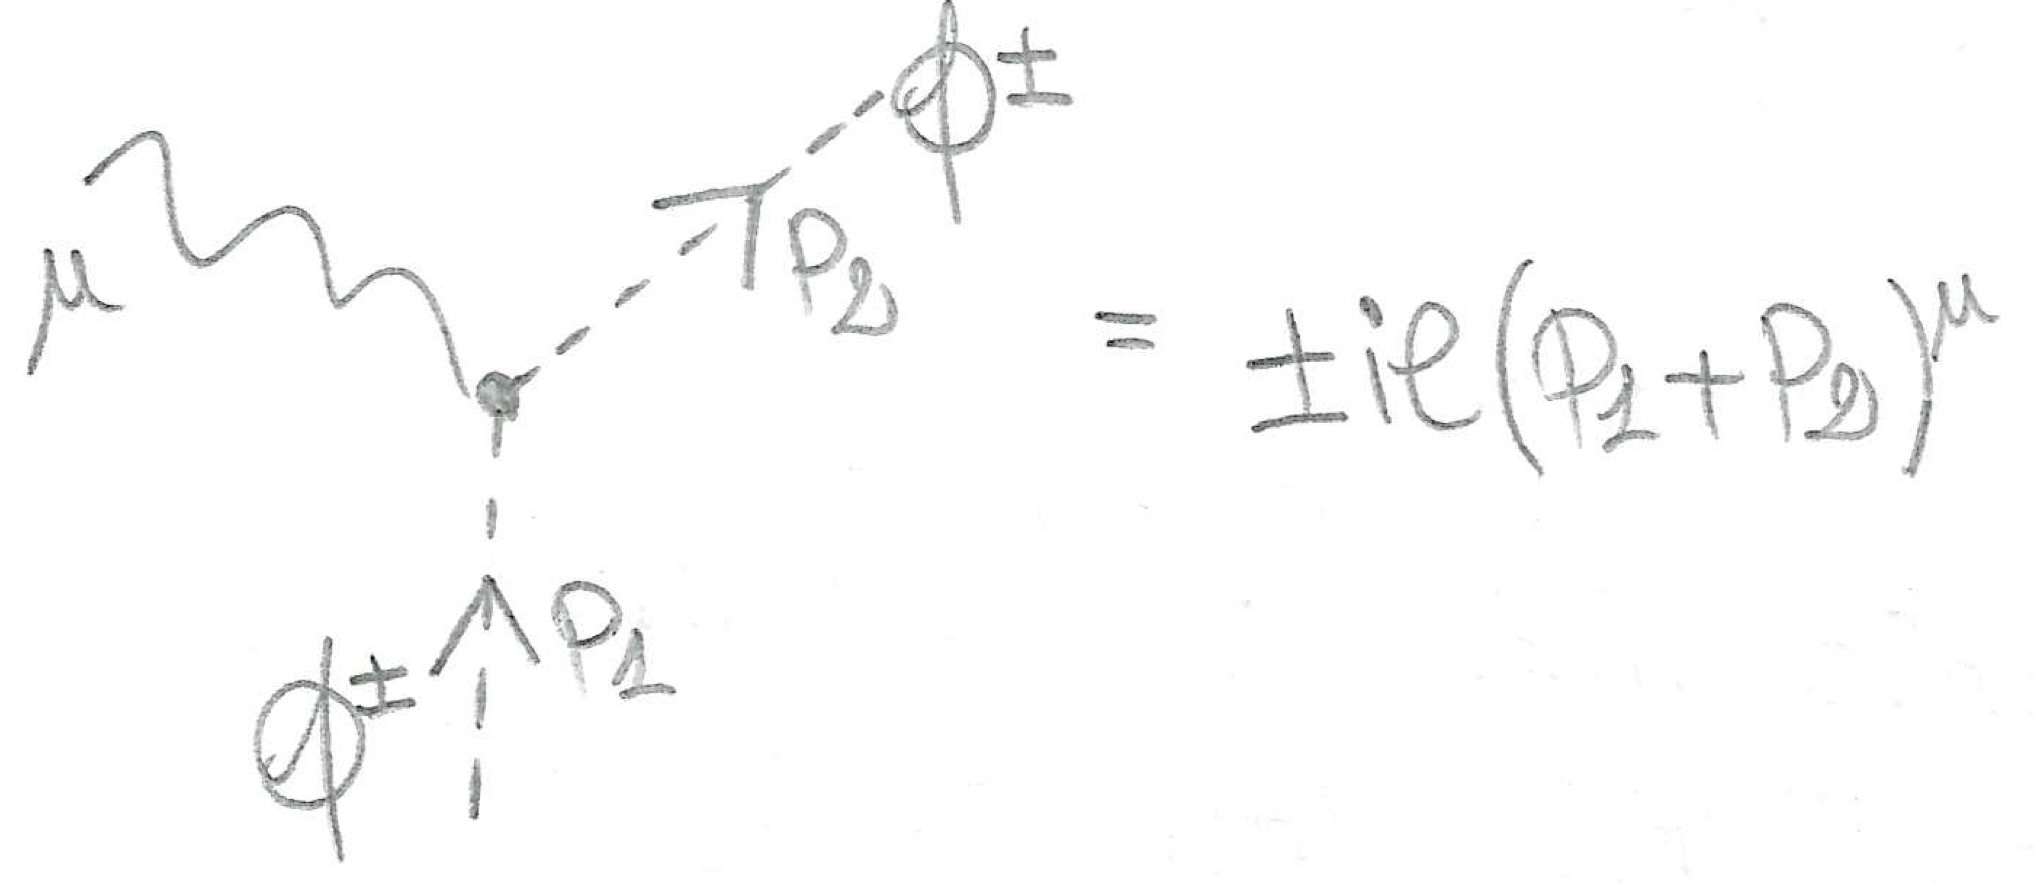
\includegraphics[]{images/vertex_feyn.jpg}

    In generale, se il vertice di interazione di tipo $i$ ha $\delta_i$ derivate, allora questo contribuirà con $\delta_i$ potenze  di impulso al power counting.
    
\end{example}

Indichiamo inoltre con:

\begin{tabular}{c|c|}
            \hline
             $P_f$           &  Numero di propagatori di tipo "$f$"\cellcolor{gray!25}  \\ \hline
             $N_f$           &  Numero di linee esterne di tipo "$f$"\cellcolor{gray!25}   \\  \hline
             $V_i$           &  Numero di vertici di interazioni di tipo "$i$"\cellcolor{gray!25}   \\ \hline
\end{tabular}

\begin{kaobox}
Indichiamo con la seguente notazione la dipendenza dall'impulso del propagatore di tipo "$f$" nello spazio dell'impulso:
\[
\Delta_f(p)\propto p^{2S_f-2} ~ \text{con} \, 
\begin{cases} 
S_f=0 \,~ \text{per fotoni e scalari} \\
S_f=\frac{1}{2} \,~ \text{per i fermioni} 
\end{cases}
\]
\end{kaobox}

Possiamo allora generalizzare l'equazione (\ref{eq:D_loop_propagators}) per il grado di divergenza superficiale (in 4 dimensioni) come segue:

\begin{equation}
    D = 4L+\sum_f (2S_f-2)P_f + \sum_i \delta_i V_i
    \label{eq:generalized_D_loop_propagators_vertices}
\end{equation}

Il numero dei loop è dato dalla generalizzazione dell'equazione (\ref{eq:L_propagators_vertices}):
\begin{equation}
    L = \sum_f P_f - \bigg(\sum_i V_i - 1\bigg)
    \label{eq:generalized_L_propagators_vertices}
\end{equation}

Sostituendo la (\ref{eq:generalized_L_propagators_vertices}) nella (\ref{eq:generalized_D_loop_propagators_vertices}) possiamo eliminare la dipendenza dal numero dei loop in $D$, ottenendo: 
\begin{equation}
    D = \sum_f 2(S_f+1)P_f + \sum_i (\delta_i - 4)V_i + 4
    \label{eq:generalized_D_propagators_vertices}
\end{equation}

\begin{kaobox}
Indichiamo con $n_{i,f}$ il numero di campi di tipo "$f$" nel vertice di interazione di tipo "$i$".
\end{kaobox}

Possiamo generalizzare le espressioni per il numero dei vertici ottenibili dalle (\ref{eq:propagators}) considerando un diagramma con un numero totale di vertici $\sum_iV_i$:
\begin{itemize}
    \item Il numero di campi di tipo "$f$" nel diagramma sarà $\sum_i V_i n_{i,f}$.
    \item Se consideriamo $N_f$ linee esterne di tipo "$f$", le rimanenti linee $\sum_i V_i n_{i,f} - N_f$ saranno chiuse in propagatori, ognuno comprensivo di due linee.
\end{itemize}

Otteniamo quindi un numero di equazioni pari al numero di diverse tipologie di campi considerate:
\begin{equation}
    \sum_i V_i n_{i,f} - N_f = 2P_f
    \label{eq:generalized_propagators}
\end{equation}
È evidente come nel caso del vertice di QED, dove $n_e = 2$ ed $n_\gamma=1$, ci si riconduca alle (\ref{eq:propagators}).

A questo punto basta risolvere per $P_f$ e sostituire nella (\ref{eq:generalized_D_propagators_vertices}) e con un po' di algebra banale si trova:
\begin{equation}
    D = 4 - \sum_f N_f(S_f+1) - \sum_i V_i [4-\delta_i-\sum_f n_{i,f}(S_f+1)]
    \label{eq:generalized_D_ext_vertices}
\end{equation}

\begin{nota}
    Nel caso del vertice di QED, tralasciando l'indice “$i$”, abbiamo $\delta=0, ~ n_e=2, ~ n_\gamma=1, ~ S_e=\frac{1}{2}, ~ S_\gamma=0$. Dunque la dipendenza dal numero dei vertici scompare e ci si riconduce alla (\ref{eq:DoD_QED_4d}).
    \label{note:qed_vertex_dependence}
\end{nota}


\begin{nota}
    Come abbiamo visto durante la trattazione legata all'equazione (\ref{eq:generalized_degree_divergence}), il coefficiente del numero dei vertici è fondamentale per determinare la rinormalizzabilità della teoria. Ciò che è interessante esplicitare è il significato intrinseco dietro questa apparente sequenza di lettere e numeri.

    Vedremo a breve che il termine tra parentesi quadre, infatti, non è altro se non (\textbf{ATTENZIONE, SPOILER}) la \textit{dimensione di massa} del coupling legato all'interazione!
    \label{note:coupling_mass_dim}
\end{nota}

\subsubsection{Parentesi: Dimensione di massa}
Consideriamo un vertice di tipo "$i$": in termini di densità di Lagrangiana corrisponderà ad un operatore con una struttura del tipo:
\begin{equation}
\mathscr{L} \supset \mathsf g_i\partial^{\delta_i}\prod_f\phi_f^{n_{i,f}}
\label{eq:lagr_vertex}
\end{equation}
dove $\mathsf g_i$ rappresenta il coupling dell'interazione e dettagli al momento irrilevanti come indici di Lorentz o come le derivate agiscono sui diversi campi sono omessi.

Nel caso della QED, considerato poco fa nella nota \ref{note:qed_vertex_dependence}, in cui $\mathsf g_\text{QED} = e$, abbiamo:
\[
\mathscr{L}_\text{QED} \supset ieA_\mu[(\partial_\mu\phi)^*\phi-\phi^*(\partial_\mu\phi)]
\]
Siccome lavoriamo in unità naturali, è noto che a livello dimensionale $[L]=[T]=[M]^{-1}$, così come $[E]=[M]$.

Una conseguenza di ciò è il fatto che, siccome vogliamo che l'azione sia adimensionale, allora dalla sua espressione in termini della densità di Lagrangiana
\[
 S = \int d^4x \mathscr{L} 
\]
troviamo che, essendo $[d^4x] = [L]^4$, $[\mathscr{L}]=[L]^{-4} = [M]^4$.

Dalla dimensione di massa della Lagrangiana possiamo quindi determinare la dimensione di massa dei principali campi per mezzo dei termini cinetici:
\begin{itemize}
    \item \textbf{Campo Fermionico}\\
          \[
          \mathscr{L} \supset i\bar\psi\gamma^\mu(\partial_\mu\psi) \Rightarrow \boxed{[\psi] = [M]^{\frac{3}{2}}}
          \]
          essendo $[\partial_\mu]=[L]^{-1}=[M]$
    \item \textbf{Campo Fotonico}
          \[
          \mathscr{L} \supset -\frac{1}{4}F_{\mu\nu}F^{\mu\nu} \supset (\partial_\mu A_\nu)(\partial^\mu A^\nu) \Rightarrow \boxed{[A_\mu] = [M]}
          \]
    \item \textbf{Campo Scalare}
          \[
          \mathscr{L} \supset \frac{1}{2}(\partial_\mu \phi)(\partial^\mu \phi) \Rightarrow \boxed{[\phi] = [M]}
          \]
\end{itemize}

In sintesi, possiamo racchiudere questi risultati in una singola equazione per un generico campo di tipo "$f$":

\begin{equation} 
[\phi_f]=[M]^{S_f+1} ~ \text{con} ~
\begin{cases}
    S_f=0 ~ \text{per fotoni e scalari}\\
    S_f=\frac{1}{2} ~ \text{per i fermioni}
\end{cases}
\label{eq:field_mass_dim}
\end{equation}

\begin{exercise}
    Dimostrare l'equazione (\ref{eq:field_mass_dim}) usando il fatto che il propagatore scala come $\Delta_f(p)\propto p^{2S_f-2}$. [\textbf{svolto lezione 3 p.42}]
\end{exercise}

Applicando quanto appena visto al caso generale in equazione (\ref{eq:lagr_vertex}) arriviamo finalmente alla dimensione di massa del coupling di interazione:
\begin{equation}
[\mathsf g_i] = [M]^{\Delta_i},~ \Delta_i=4-\delta_i-\sum_f n_{i,f}(S_f+1)
\label{eq:coupling_mass_dim}
\end{equation}
Come preannunciato nella nota \ref{note:coupling_mass_dim}, la dimensione di massa del coupling è esattamente il coefficiente che moltiplica il numero dei vertici nell'espressione generalizzata del grado di divergenza superficiale!

Per coronare quanto appena appreso, riscriviamo l'equazione (\ref{eq:generalized_D_ext_vertices}) in maniera più elegante:
\begin{equation}
    D = 4 - \sum_f N_f(S_f-1) - \sum_i V_i \Delta_i
    \label{eq:generalized_D_coupling_massdim}
\end{equation}

È notevole (ed estremamente soddisfacente) come \textbf{dalla dimensione di massa della costante di accoppiamento dell'interazione si possa determinare la rinormalizzabilità della teoria}:
\begin{itemize}
    \item Se $\Delta_i>0 ~\forall ~ i = 1,...,n_I$ abbiamo una teoria super-rinormalizzabile, in quanto solo un numero finito di diagrammi diverge.
    \item Se $\Delta_i \geq 0 ~\forall ~ i$ e almeno un $\Delta_j = 0$, la teoria è rinormalizzabile, in quanto almeno un'ampiezza perderà la dipendenza dal numero dei vertici nel grado di divergenza e genererà un'infinità di diagrammi divergenti.
    \item Se almeno un $\Delta_i < 0$, la teoria non è rinormalizzabile, in quanto avremmo un numero infinito di ampiezze divergenti.
\end{itemize}

\begin{exercise}
    Generalizzare l'equazione (\ref{eq:generalized_D_coupling_massdim}) in un arbitrario numero "$\mathsf{d}$" di dimensioni spazio-temporali. [\textbf{svolto lezione 3 p.44}]\\
    
    \textbf{Risultato:}
    \begin{equation}
    \boxed{
    \begin{aligned}
    D &= \mathsf{d} - \sum_f N_f\bigg(S_f - 1 - \frac{\mathsf{d}}{2}\bigg) - \sum_i V_i \Delta_i \\
      &\text{con}~\Delta_i = \mathsf{d}\bigg(1-\frac{1}{2}\sum_f n_{i,f}\bigg)- \delta_i - \sum_f  n_{i,f}(S_f-1)
    \end{aligned}
    }
    \label{eq:ex142_sol}
    \end{equation}
\end{exercise}

\begin{kaobox}
    \textbf{Fatto Generico:}
    \begin{itemize}
        \item Quando $\mathbf{\mathsf{d}>4}$, la maggioranza delle teorie che sono rinormalizzabili in 4 dimensioni diventano non rinormalizzabili.
        \item Quando $\mathbf{\mathsf{d}<4}$, teorie non rinormalizzabili in 4 dimensioni diventano rinormalizzabili.
    \end{itemize}
\end{kaobox}

\subsection{Osservazioni finali // Dimensioni}
In QFT, la QED in $\mathsf{d}$-dimensioni è data dall'azione:
\[
S = \int d^\mathsf{d}x \bigg[-\frac{1}{4}F_{\mu\nu}F^{\mu\nu} + \bar\psi(i\slashed\partial - m)\psi + e\bar\psi\slashed A\psi \bigg]
\]
dove si è adottata la slash-notation di Dirac: $\slashed X = \gamma^\mu X_\mu$.

Di conseguenza possiamo ricavare:
\begin{itemize}
    \item \textbf{La dimensione di massa dei campi}
        \[
        [\psi] = [M]^{\frac{\mathsf{d}-1}{2}} ~,~ [A^\mu] = [M]^{\frac{\mathsf{d}}{2}-1}
        \]

    \item \textbf{La dimensione di massa del coupling}
        \[
        [e] = [M]^{2 - \frac{\mathsf{d}}{2}} \Rightarrow \boxed{\Delta_e = 2 - \frac{\mathsf{d}}{2}}
        \Rightarrow \begin{cases}
                    \mathsf{d} = 4 \Rightarrow \Delta_e = 0 ~(\text{RIN})\\
                    \mathsf{d} < 4 \Rightarrow \Delta_e > 0 ~(\text{SUPER-RIN})\\
                    \mathsf{d} > 4 \Rightarrow \Delta_e < 0 ~(\text{NON-RIN})
            \end{cases}
        \]
    \item \textbf{L'integrale al loop nello spazio dell'impulso}
        \[
        \int \frac{d^4k}{(2\pi)^4} \rightarrow \int \frac{d^\mathsf{d}k}{(2\pi)^4}
        \]
\end{itemize}

    \begin{nota}
        Si può mostrare come l'equazione di Dirac $\mathsf{d}$-dimensionale mantenga la stessa struttura di quella in 4 dimensioni. Chiaramente la fisica è completamente differente! [\textbf{Lezione 4, p.48÷53}]
    \end{nota}

\subsection{Osservazioni finali // Teorie}
\[
D = 4 - \sum_f N_f(S_f-1) - \sum_i V_i \Delta_i 
\Rightarrow \begin{cases}
                \Delta_e > 0 ~ (\textcolor{Green}{\text{Super-Rinormalizzabile}})\\
                 \Delta_e = 0 ~ (\textcolor{Blue}{\text{Rinormalizzabile}})\\
                 \Delta_e < 0 ~ (\textcolor{Red}{\text{Non-Rinormalizzabile}})
            \end{cases}
\]
\begin{itemize}
    \item \textbf{Teorie Scalari}\\
    
    \begin{tabular}{|c|c|c|}
            \hline
             $\lambda\phi^3$ \cellcolor{green!25}          &  $\lambda\phi^4$\cellcolor{blue!25}  & $\lambda\phi^5$ ... \cellcolor{red!25}\\ \hline
             $\Delta_\lambda = 1$           &  $\Delta_\lambda = 0$ & $\Delta_\lambda \leq -1$ \\ 
            \hline
\end{tabular}\\

    \item \textbf{Scalari + Fermioni}\\
    
    \begin{tabular}{|c|c|c|}
            \hline
             $y\phi\bar\psi\psi$ \cellcolor{blue!25}       &  $y\phi\bar\psi\gamma^5\psi$\cellcolor{blue!25}  & $y(\partial_\mu\phi)\bar\psi\gamma^\mu\psi$ \cellcolor{red!25}\\ \hline
             $\Delta_\lambda = 0$           &  $\Delta_\lambda = 0$ & $\Delta_\lambda = -1$ \\ 
            \hline
\end{tabular}\\

    \item \textbf{Scalari + Fermioni + Campi di Gauge}\\
    
        \begin{tabular}{|c|c|c|c|c|}
            \hline
             $\mathsf g\bar\psi\gamma^\mu\psi A_\mu$ \cellcolor{blue!25}       &  $\mathsf g\bar\psi\gamma^\mu\gamma^5\psi A_\mu$\cellcolor{blue!25}  &  $\mathsf g(\phi^*\partial_\mu\phi - \phi\partial_\mu\phi^*) A_\mu$ \cellcolor{blue!25} & $\mathsf g \phi^2A_\mu A^\mu$\cellcolor{blue!25} & $\mathsf g F_{\mu\nu}\bar\psi\sigma^{\mu\nu}\psi$\cellcolor{red!25}\\ \hline
             $\Delta_\mathsf g = 0$           &  $\Delta_\mathsf g = 0$ & $\Delta_\mathsf g = 0$ & $\Delta_\mathsf g = 0$ & $\Delta_\mathsf g = -1$ \\ 
            \hline
\end{tabular}
    
\end{itemize}

\end{document}


\begin{figure}[h]
    \centering
    \includegraphics{images/semplicementepanati.png}
    \caption*{}
    \label{fig:my_label}
\end{figure}